\documentclass[a4paper,12pt,oneside]{book}
\usepackage{pdfpages}
\usepackage{polski}
\usepackage{fancyhdr}
\usepackage{graphicx}
\usepackage{pgf-pie}
\usepackage{float}
\usepackage{caption}
\usepackage{subcaption}
\usepackage{listings}
\usepackage[utf8]{inputenc}
\usepackage{amsthm}
\usepackage[intlimits]{amsmath}
\usepackage{cite}


\lstdefinelanguage{JavaScript}{
	keywords={typeof, new, true, false, catch, function, return, null, catch, switch, let, if, in, while, do, else, case, break, const},
	keywordstyle=\color{blue}\bfseries,
	ndkeywords={class, export, boolean, throw, implements, import, this},
	ndkeywordstyle=\color{darkgray}\bfseries,
	identifierstyle=\color{black},
	sensitive=false,
	comment=[l]{//},
	morecomment=[s]{/*}{*/},
	commentstyle=\color{purple}\ttfamily,
	stringstyle=\color{red}\ttfamily,
	morestring=[b]',
	morestring=[b]"
}

\lstset{
	language=JavaScript,
	backgroundcolor=\color{white},
	extendedchars=true,
	basicstyle=\footnotesize\ttfamily,
	showstringspaces=false,
	showspaces=false,
	numbers=left,
	numberstyle=\footnotesize,
	numbersep=9pt,
	tabsize=2,
	breaklines=true,
	showtabs=false,
	captionpos=b
}

\linespread{1.25}
\pagestyle{fancy}
\fancyhf{}
\fancyhead[LO]{\footnotesize\rightmark}
\fancyhead[RE]{\footnotesize\leftmark}
\fancyhead[LE,RO]{\footnotesize\thepage}
\begin{document}
	\thispagestyle{empty}
	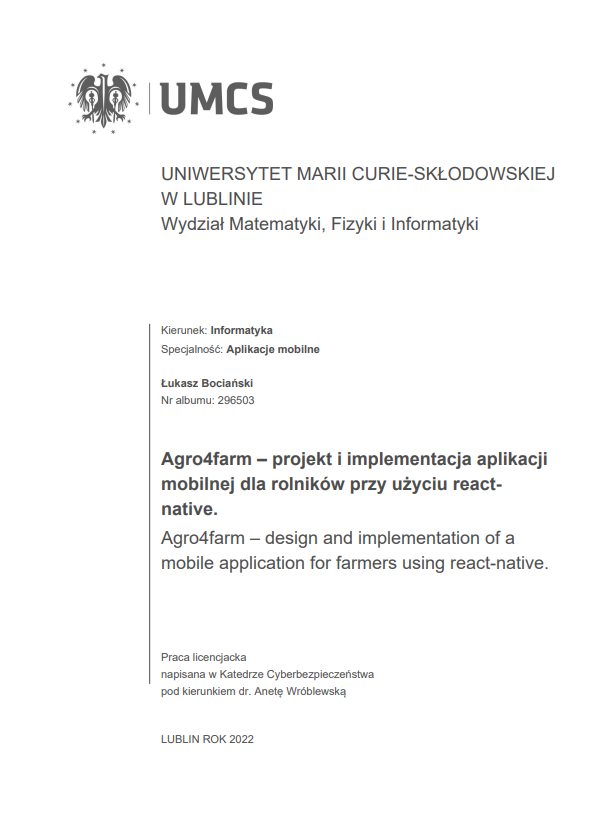
\includepdf{stronatytulowa}
	
	\newpage
	\thispagestyle{empty}
	\
	
	\newpage
	\thispagestyle{empty}
	\chapter*{Streszczenie}
		\ \ \ Rolnictwo jest obszarem gospodarki prężnie rozwijającym się w ostatnich latach. W ramach niniejszej pracy zaprojektowano oraz stworzono aplikację mobilną dla rolników oraz dokładnie przedstawiono wszystkie jej funkcjonalności wraz z użytymi w niech technologiami. Oprócz tego została opisana krótka historia urządzeń mobilnych wraz z mobilnymi systemami operacyjnymi. Przedstawiono również narzędzia używane w rolnictwie, a także dostępne na rynku aplikacje dla rolników.
			
		\textbf{Słowa kluczowe:} \textit{aplikacja mobilna, rolnictwo, react native}
	
		\newpage
	\thispagestyle{empty}
	\chapter*{Abstract}
		\ \ \ Agriculture is an area of the economy that has been growing rapidly in recent years. In this paper a mobile application for farmers has been designed and all its functionalities along with the technologies used in it have been presented in detail. In addition, a brief history of mobile devices along with mobile operating systems was described. The tools used in agriculture are also presented, as well as the applications for farmers available on the market.
		
		\textbf{Keywords:} \textit{mobile application, farming, react native}
	
	\newpage
	\thispagestyle{empty} %usuń styl (fancyheader)
	\tableofcontents %spis tresci
	
	\newpage
	\thispagestyle{empty}
	\chapter*{Wstęp} %bez numeru
	
		\ \ \ \ \ Rolnictwo jest zawodem, którego historia sięga początków ludzkości. Przez tysiące lat dzięki pomysłowości ludzi tworzono coraz nowsze sposoby na ułatwienie pracy na roli. Od prostych narzędzi i wykorzystywania zwierząt, aż do nowoczesnych maszyn oraz specjalistycznych nawozów, rolnictwo ewoluowało i nadal ewoluuje. Większość społeczeństwa uważa rolników za osoby wykonujące ciężką i brudną robotę bez wiedzy na temat nowych technologii. Nie jest to do końca prawda, gdyż ten stereotyp jest widoczny w starym pokoleniu rolników. Coraz więcej młodych właścicieli gospodarstw zaczyna używać nowych narzędzi oraz technologii, które znacznie przyśpieszają i ułatwiają ich już wystarczająco ciężką pracę.
		
		Główną częścią niniejszej pracy jest przedstawienie rozwiązania opracowanego dla rolników, czyli aplikacji mobilnej "Agro4Farm". Oprócz szczegółowych opisów poszczególnych funkcji oraz użytych w nich technologii, przedstawiono krótką historię urządzeń mobilnych oraz pokazano dostępne na rynku aplikacje stworzone dla osób pracujących na roli.
	
	\addcontentsline{toc}{chapter}{Wstęp}
	
	\newpage
	\thispagestyle{empty}
	\chapter{Urządzenia mobilne}
	\section{Początki urządzeń mobilnych}
	\ \ \ \
	Nie da się ukryć, że w dzisiejszych czasach wszelka technologia rozwija się w zawrotnym tempie. W przeciągu ostatnich siedmiu dekad na rynek wchodziły coraz nowsze urządzenia elektroniczne mające na celu ułatwienie dostępu do informacji oraz do kontaktu między ludźmi. Pierwsze prototypy telefonów komórkowych zaczęły się pojawiać w latach pięćdziesiątych dwudziestego wieku, kiedy to szwedzka firma Ericson zaprezentowała pierwszy przenośny telefon ważący około 40 kilogramów, a kształtem przypominający walizkę. W 1973 roku firma Motorola wprowadziła do sprzedaży Motorolę DynaTAC 8000X \cite{ref1}. Telefon ten porównać można było do cegły głownie przez jego wagę oraz rozmiar, a wzorowany był na urządzeniu używanym przez bohatera popularnej serii "Star Trek". Urządzenie niczym nie przypominało telefonów produkowanych w dzisiejszych czasach. Jego bateria wystarczyła na zaledwie 30 minut rozmów, a naładowanie go trwało około 10 godzin. 
	
	Przez następne lata, na rynek trafiały coraz to nowsze urządzenia oraz technologie produkowane przez firmy takie jak: Nokia, IBM, Motorola czy Siemens. Początki dwudziestego pierwszego wieku to okres, w którym urządzenia mobilne przeszły w nową epokę, a mowa tu dokładniej o pierwszych telefonach dotykowych.
	
	\section{Pierwsze smartfony}
	\ \ \ 
	Smartfon to inaczej przenośne urządzenie posiadające w sobie funkcje telefonu komórkowego oraz komputera osobistego. Pierwsze pomysły na ich stworzenie pojawiły się w 1992 roku. Prototyp takiego urządzenia został zaprezentowany przez firmę IBM. Pozwalał on na prowadzenie rozmów, wysyłanie faxów i poczty elektronicznej oraz przeglądanie stron internetowych. Było to dosyć prymitywne urządzenie o dużych rozmiarach. Prawdziwym przełomem okazał się rok 2007, kiedy to 9 stycznia firma Apple zaprezentowała swój pierwszy iPhone, który zawitał na rynku pół roku później.
	
	\begin{figure}[h]
		\centering
		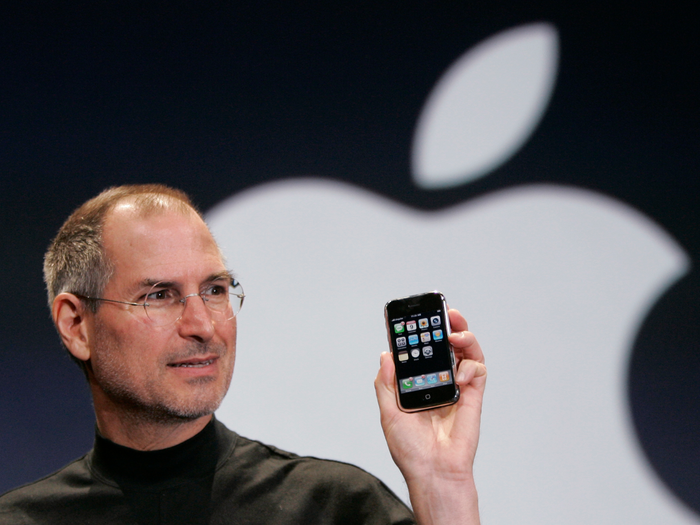
\includegraphics[width=0.75\textwidth]{grafika/steve_jobs_iphone_presentation.png}
		\caption{Steve Jobs prezentujący pierwszy model iPhone}
	\end{figure}
	
	Wprowadzenie iPhone na rynek był gigantycznym skokiem w technologii. Ciężko było w jakikolwiek sposób z nim konkurować, ponieważ urządzenie to swoją konstrukcją, prostotą użycia oraz funkcjonalnościami przyćmiewała inne urządzenia. Producenci zrezygnowali z dosyć popularnych funkcjonalności, które były popularne w tamtych czasach. Klawiaturę zastąpiono ekranem dotykowym, a samo urządzenie posiadało 3,5 calowy ekran oraz przycisk "Home" \cite{ref2}. 
	\newpage
	Na dzień premiery iPhone posiadał wiele więcej rewolucyjnych funkcjonalności takich jak:
	
	\begin{description}
		\item[Klawiatura ekranowa -] pozwalającą na wprowadzanie danych przez klawiaturę używając ekranu dotykowego. Funkcja ta posiadała również korektę dotknięć, która ignorowała przypadkowe kliknięcia na ekranie.
		\item[Czujnik zbliżeniowy -] który wyłączał ekran podczas gdy użytkownik zbliżył twarz do ekranu urządzenia.
		\item[Nowoczesna przeglądarka internetowa -] która pozwalała na wykorzystanie pełni możliwości języka HTML.
		\item[Multitouch -] czyli możliwość wykrywania przez ekran dotykowy wielu jednoczesnych kliknięć.
		\item[Żyroskop -] czyli funkcja wykrywająca stopień pochylenia urządzenia. 
	\end{description}

	Kolejne lata można nazwać "wyścigiem technologicznym", w którym to firmy konkurowały ze sobą tworząc coraz nowsze urządzenia oraz rozwijały istniejące już technologie w celu dorównania do wymogów konsumentów.
	
	\begin{figure}[h]
		\centering
		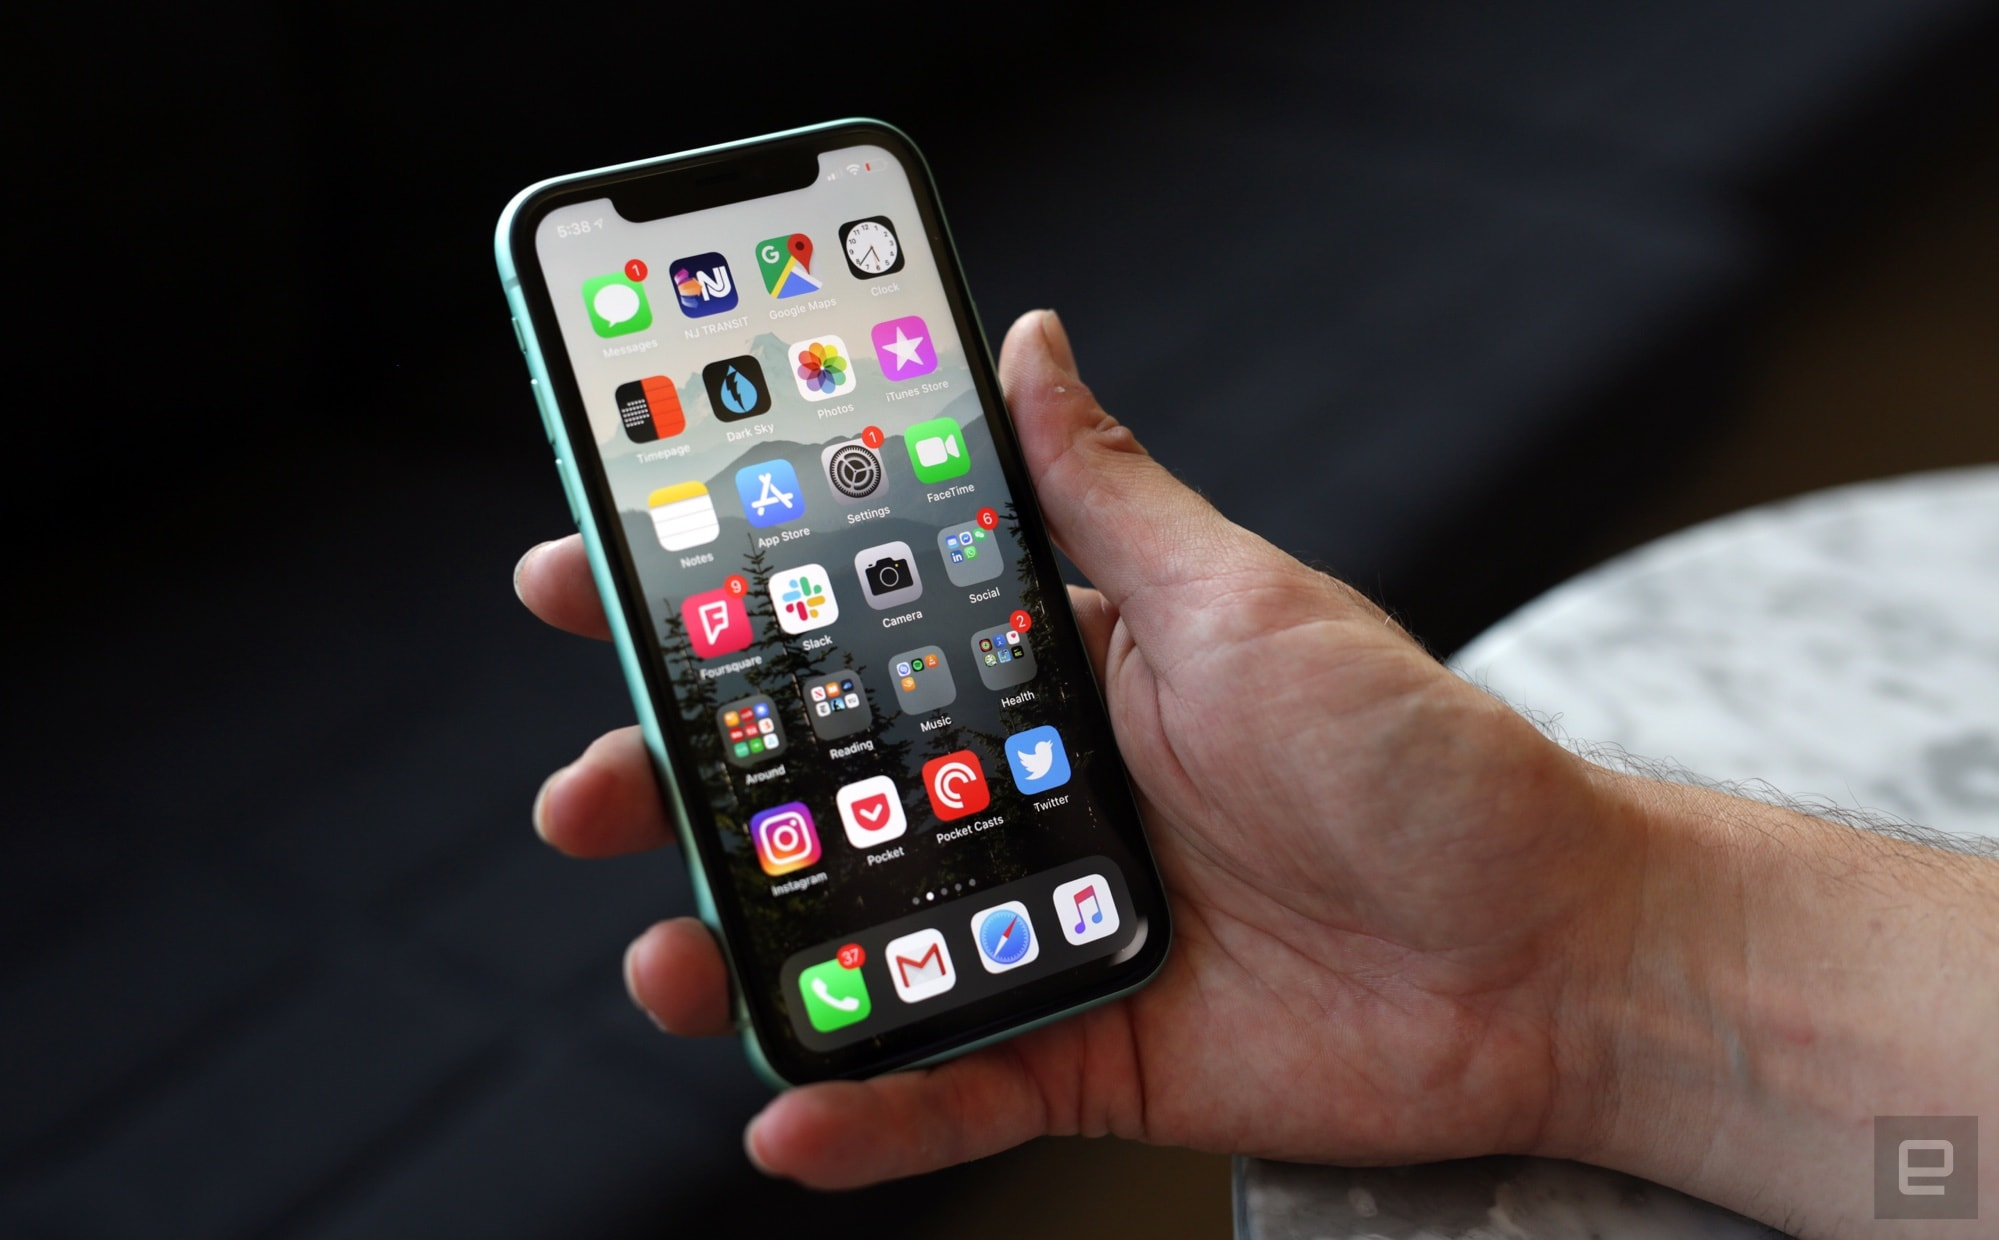
\includegraphics[width=0.75\textwidth]{grafika/iphone11}
		\caption{Model iPhone 11 wydany w 2019r}
	\end{figure}
	
	\newpage
	\section{Smartfony w dzisiejszych czasach}
	\ \ \ \
	Dziś liczba producentów na rynku produkujących urządzenia mobilne jest spora i dalej rośnie. W ciągu ostatnich piętnastu lat pojawiali się nowi producenci smartfonów razem ze swoimi innowacyjnymi pomysłami ulepszającymi swoje poprzednie urządzenia. 
	
	\begin{figure}[h]
		\centering
		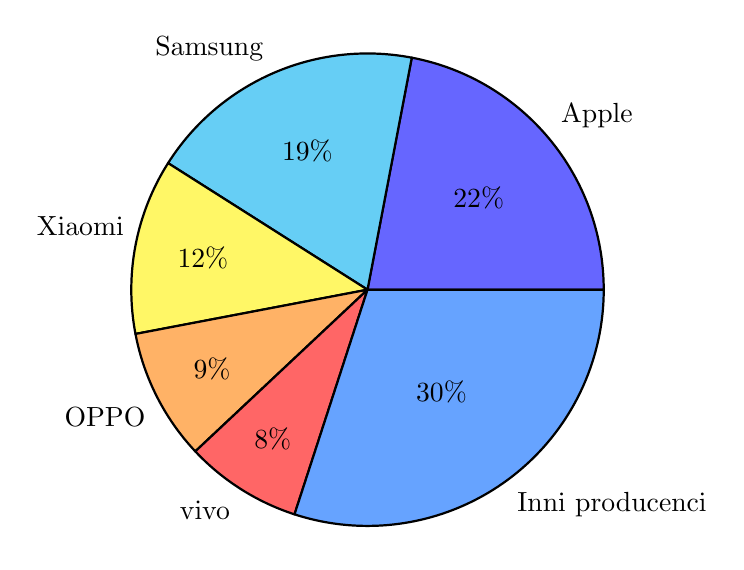
\begin{tikzpicture}
			\pie[radius=3]{22/Apple,
				19/Samsung,
				12/Xiaomi,
				9/OPPO,
				8/vivo,
				30/Inni producenci}
		\end{tikzpicture}
		\caption{Udział w globalnym rynku dostaw smartfonów, 4 kwartał 2021r}
	\end{figure}
	
	Jak widać na załączonym wyżej wykresie (Rysunek 1.3), globalnym liderem rynkowym nadal pozostaje Apple wraz ze swoim flagowym produktem iPhone. Na drugim i trzecim miejscu utrzymują się firmy Samsung oraz Xiaomi. Można więc wywnioskować, że wzrost liczby producentów oraz urządzeń dostępnych na rynku jak i coraz niższe ceny telefonów, przekładają się na korzystniejszą dostępność oraz większą popularność danych modeli \cite{ref3}. 
	
	W wynikach badań przeprowadzonych przez CBOS (Centrum Badania Opinii Społecznej) z 2021 roku, w których sprawdzano jak na przestrzeni lat zmieniała się popularność telefonów posiadanych w polskich gospodarstwach domowych, zauważyć można owe zmiany w popularności urządzeń mobilnych.
	
	\newpage
	\begin{figure}[h]
		\centering
		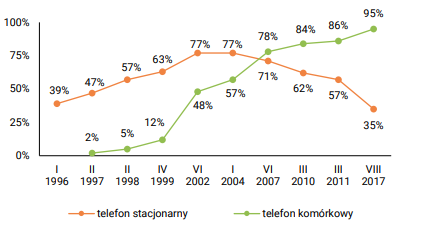
\includegraphics[width=0.75\textwidth]{grafika/cbos_wykres.png}
		\caption{Telefony w gospodarstwach domowych w latach 1996-2017}
	\end{figure}

	Jak widać na przedstawionym wykresie (Rysunek 1.4) \cite{ref4}, urządzenia mobilne zaczęły dosyć szybko stawać się popularne. Początkiem popularności telefonów komórkowych nad telefonami stacjonarnymi był rok 2007, kiedy to, jak już wcześniej było wspomniane, do sprzedaży wprowadzono pierwszy model iPhone. Rok ten można nazwać początkiem ery nowych urządzeń mobilnych. Sam wybór między klasycznym telefonem komórkowym, a smartfonem jest w głównej mierze uwarunkowany wiekiem i grupą społeczną użytkownika.
	
	\begin{figure}[h]
		\centering
		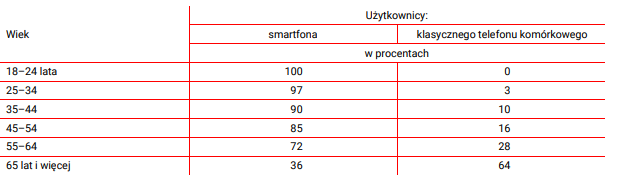
\includegraphics[width=1\textwidth]{grafika/cbos_wykres2.png}
		\caption{Procent wyboru klasycznych telefonów komórkowych i smartfonów w różnych przedziałach wiekowych}
	\end{figure}

	\newpage

	Powyższa tabela (Rysunek 1.5) \cite{ref4} pokazuje preferencje wyboru telefonów wśród użytkowników względem ich wieku. Dla osób w wieku od 18 do 24 lat najbardziej popularne są smartfony. Liczba ta z każdą kategorią wiekową maleje. Dzieje się tak dlatego, że młodsze społeczeństwo jest bardziej przyswojone do zmian i nowości technologicznych, w przeciwieństwie do starszego społeczeństwa.
	
	\section{Smartfony i inne technologie używanie w rolnictwie}
	\ \ \ \
	Jak już wcześniej zostało wspomniane, jednymi z głównych czynników w tym czy dana osoba chętniej korzysta z urządzeń mobilnych jest wiek oraz grupa społeczna. Wśród najczęstszych posiadaczy smartfonów można wyróżnić studentów, uczniów szkół, pracowników biurowych oraz specjalistów z wyższym wykształceniem. Można więc dojść do wniosku, że urządzenia typu smartfon w większości są używane przez osoby kształcące się oraz przez osoby wykonujące pracę umysłową. Rolnicy natomiast są zaliczani do grupy osób wykonujących prace czysto fizyczną. Większość osób uważa rolników za osoby nie posiadające większej wiedzy na temat nowoczesnych technologii. Nic bardziej mylnego. Na przełomie ostatnich lat, rolnictwo ewoluowało i przyswajało coraz to nowsze technologie. Można powiedzieć, że smartfony stały się podstawowym narzędziem rolników. Dzięki nim rolnicy są w stanie używać nowych technologii takich jak:
	
	\begin{description}
		\item[Drony -] sterowane za pomocą telefonów, pozwalają na doglądanie upraw z lotu ptaka, tworzenia precyzyjnych map pól, a nawet nawożenie upraw środkami do ochrony roślin.
		\item[Czujniki upraw -] które ułatwiają kontrolę upraw oraz pozwalają na skuteczne dawkowanie nawozów.
		\item[GPS -] przy pomocy którego można dokumentować stan gruntów rolnych oraz mapować pola.
		\item[Aplikacje mobilne -] pozwalają one na łatwe zarządzanie gospodarstwem za pomocą smartfonów. Rolnik może używać ich w każdej chwili, przechowywać ważne informacje, używać ich do sprawdzania warunków pogodowych, robić notatki, planować pracę oraz wiele więcej.
	\end{description}

	Zmiany te są bardziej widoczne wśród młodszych rolników, którzy chętniej przyswajają nowe technologie, aby dzięki nim osiągnąć lepsze wyniki produkcji, ułatwić sobie wykonywaną pracę oraz zaoszczędzić sporo czasu \cite{ref5}.
	
	\newpage
	\thispagestyle{empty}
	\chapter{Systemy i aplikacje mobilne}
	\section{Mobilne systemy operacyjne}
	\ \ \ \
	Sama nazwa "system operacyjny" kojarzona jest głównie z komputerami osobistymi. Systemy mobilne mimo tego, że w pewnym stopniu bazują na systemach operacyjnych używanych w komputerach osobistych to posiadają szereg różnic i usprawnień stworzonych głównie w celu ułatwienia użytkownikowi w posługiwaniu się urządzeniem. Szybki rozwój urządzeń mobilnych przyczynił się do stworzenia systemów takich jak Symbian, Windows Phone, BlackBerry OS, iOS czy Android, z których to właśnie te dwa ostatnie czyli iOS oraz Android są liderami używanymi w dzisiejszych czasach.
	
	\subsection{System iOS}
	\ \ \ \
	System iOS jest systemem stworzonym oraz w dalszym ciągu rozwijanym przez firmę Apple dostępnym tylko na urządzeniach tej firmy. Początkowo nazywany iPhone OS, system ten po raz pierwszy został zaprezentowany w roku 2007 przez Steava Jobsa podczas prezentacji pierwszego iPhone. System iOS bazuje na architekturze systemu Mac OS X, a ich struktura składa się z czterech abstrakcyjnych warstw (Rysunek 2.1) \cite{ref10}.
	
	\newpage
	
	\begin{figure}[h]
		\centering
		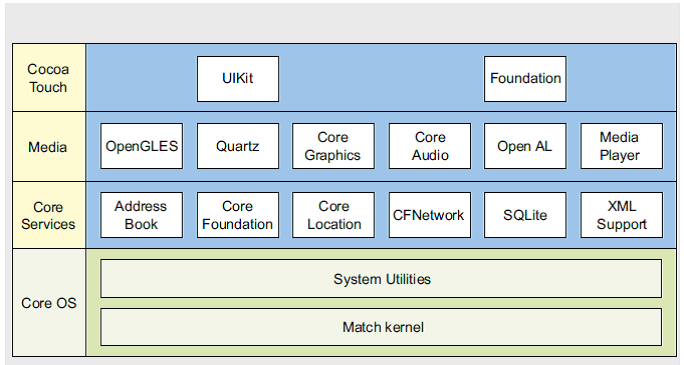
\includegraphics[width=0.85\textwidth]{grafika/warstwy_ios.png}
		\caption{Warstwy systemu iOS}
	\end{figure}

	Pierwsza warstwa, czyli "Cocoa Touch" jest biblioteką odpowiedzialną za interfejs użytkownika. Interfejs ten jest sterowany za pomocą wbudowanego ekranu dotykowego. Warstwa "Media" jest warstwą obsługującą dźwięk i obraz. W skład tej warstwy wchodzą biblioteki takie jak: OpenGLES, Quartz, Core Graphics, Core Audio, Open AL oraz Media Player. Kolejną warstwą wchodzącą w skład systemu iOS jest warstwa "Core Services". Odpowiada ona za zarządzanie aplikacjami oraz wątkami. Posiada także funkcje obsługujące sieć i bazy danych. Ostatnią z warstw jest warstwa "Core OS", która ma za zadanie zapewnienia komunikacji między urządzeniem a oprogramowaniem. Z biegiem lat powstawały nowe wersje systemu, które posiadały szereg udogodnień oraz poprawek. Obecnie istnieje szesnaście wersji systemu iOS. 
	
	\subsection{System Android}
	\ \ \ \
	W roku 2005 po przejęciu przez firmę Google firmy Android Inc, stworzony został system na urządzenia mobilne oparty na jądrze Linuxa o nazwie Android. Prototypy urządzeń wraz z systemem zostały zaprezentowane w 2008 roku na Mobile World Congres. Od tamtej pory rozwój systemu Android przyśpieszył, aby następnie w 2013 roku zostać ogłoszonym najpopularniejszym systemem mobilnym na świecie.
	
	\newpage
	Schemat systemu Android prezentuje się następująco na Rysunku 2.2 \cite{ref11} .
	
	\begin{figure}[h]
		\centering
		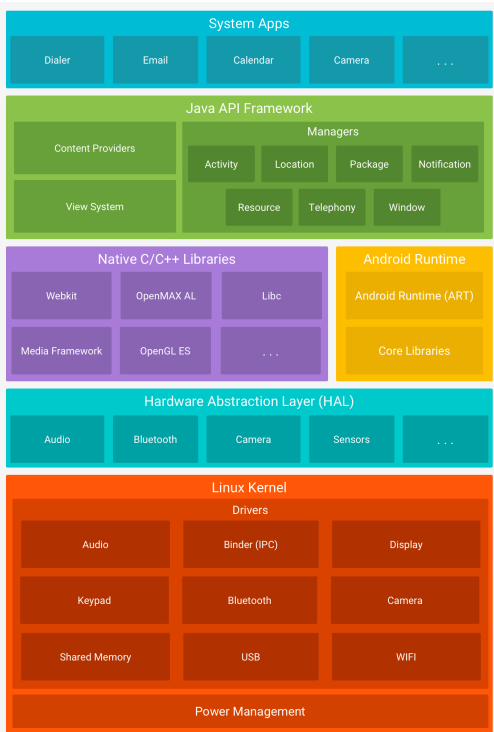
\includegraphics[width=0.70\textwidth]{grafika/schemat_android.png}
		\caption{Schemat systemu Android}
	\end{figure}
	
	System Android cechuje się wieloma zaletami, z których najważniejszymi są: elastyczność systemu, intuicyjność obsługi, mnogość nakładek systemowych, regularne aktualizacje systemowe oraz możliwość rootowania urządzenia i wrzucenia dowolnego systemu. System ten posiada również kilka wad z których największą z nich jest duża podatność na ataki. Patrząc na dzisiejszy rynek telefonów, system Android jest zdecydowanym liderem pod względem dostępności. W przeciwieństwie do systemu iOS, który jest dostępny wyłącznie na urządzeniach firmy Apple, Android jest systemem dostępnym na urządzeniach wielu różnych producentów.
	
	\section{Rozwój aplikacji mobilnych}
	\ \ \ \
	Aplikacje mobilne to rodzaj oprogramowania tworzonego z myślą o urządzeniach mobilnych. Aplikacje te podzielić można na podstawie ich zastosowania oraz grupy osób, dla której zostały one stworzone. Zdecydowanie najpopularniejszymi typami aplikacji mobilnych są aplikacje społecznościowe \cite{ref12}.
	
	\begin{figure}[h]
		\centering
		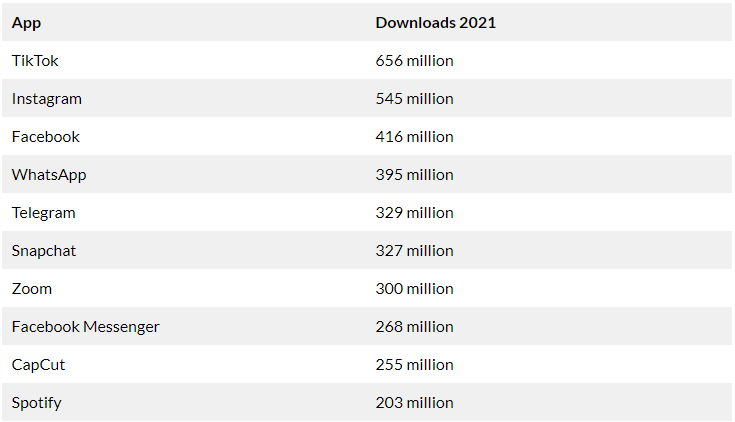
\includegraphics[width=0.9\textwidth]{grafika/most_popular_apps_2021.png}
		\caption{Lista najpopularniejszych aplikacji mobilnych w 2021 roku pod względem ilości pobrań}
	\end{figure}

	Jak widać na załączonym Rysunku 2.3 w pierwszej dziesiątce, aż osiem pozycji to aplikacje społecznościowe.  W ciągu ostatnich lat oprogramowanie mobilne ewoluowało wraz z dostępnymi na rynku urządzeniami. Wprowadzanie przez producentów nowych funkcjonalności do swoich urządzeń dawało deweloperom aplikacji na smartfony coraz większe możliwości. 
	
	\newpage
	
	Oprócz zmian na rynku aplikacji oraz urządzeń mobilnych z biegiem lat można było również zauważyć powstawanie nowych środowisk skierowanych dla programistów aplikacji mobilnych. Do tych najpopularniejszych możemy zaliczyć: Flutter, Ionic, VueJS, Mobile Angular UI, Xamarin, jQuery Mobile, NativeScript, React Native. Używają one różnych języków programowania takich jak C/C++ w przypadku Flutter, JavaScript dla React Native, VueJS i jQuery Mobile, czy C\# w Xamarin. Większość tych frameworków wspiera wieloplatformowość, gdzie aplikacje pisane są głównie z myślą o urządzeniach z Androidem oraz iOS.
	
	\section{Aplikacje dla rolników}
	\ \ \ \
	Celem tej pracy jest przedstawienie aplikacji zaprojektowanej dla rolników, dlatego nie może tu zabraknąć wzmianek o oprogramowaniu oraz rozwiązaniach dostępnych na rynku. W serwisach takich jak "Sklep Play" w łatwy sposób pobrać możemy aplikacje dla rolników, które posiadają w sobie funkcje takie jak: menadżer pola, który pozwala użytkownikowi na oznaczanie oraz zapisywanie na mapach swoich pól; aplikacje typu kalkulator, które pozwalają na obliczanie wskaźników wysiewu czy stóp kapitalizacji; aplikacje z wyszukiwarkami chorób i środków ochrony roślin.
	
	Zdecydowanie najczęściej pojawiającym się typem aplikacji w Sklepie Play, w kategorii "rolnictwo" jest nawigacja dla rolników. Przykładem takiej aplikacji jest "Nawigator polowy" \cite{ref6}. Aplikacja ta pozwala na tworzenie listy posiadanych pól oraz zarządzanie nimi. Przy użyciu map Google użytkownik może znaleźć po swojej aktualnej lokalizacji lub poprzez wpisanie adresu miejsce, w którym pole może się znajdować. Następnie, tak jak jest to przedstawione na Rysunku 2.4, użytkownik jest w stanie zaznaczyć obszar rolny na mapie, nazwać go i określić jaka uprawa się na nim znajduje. Po zapisaniu, pole zostanie dodane do listy wraz z jego opisami oraz powierzchnią. Tam rolnik jest w stanie edytować pole lub użyć opcji do nawigacji po nim.
	
	\begin{figure}[H]
		\centering
		\begin{subfigure}{.5\textwidth}
			\centering
			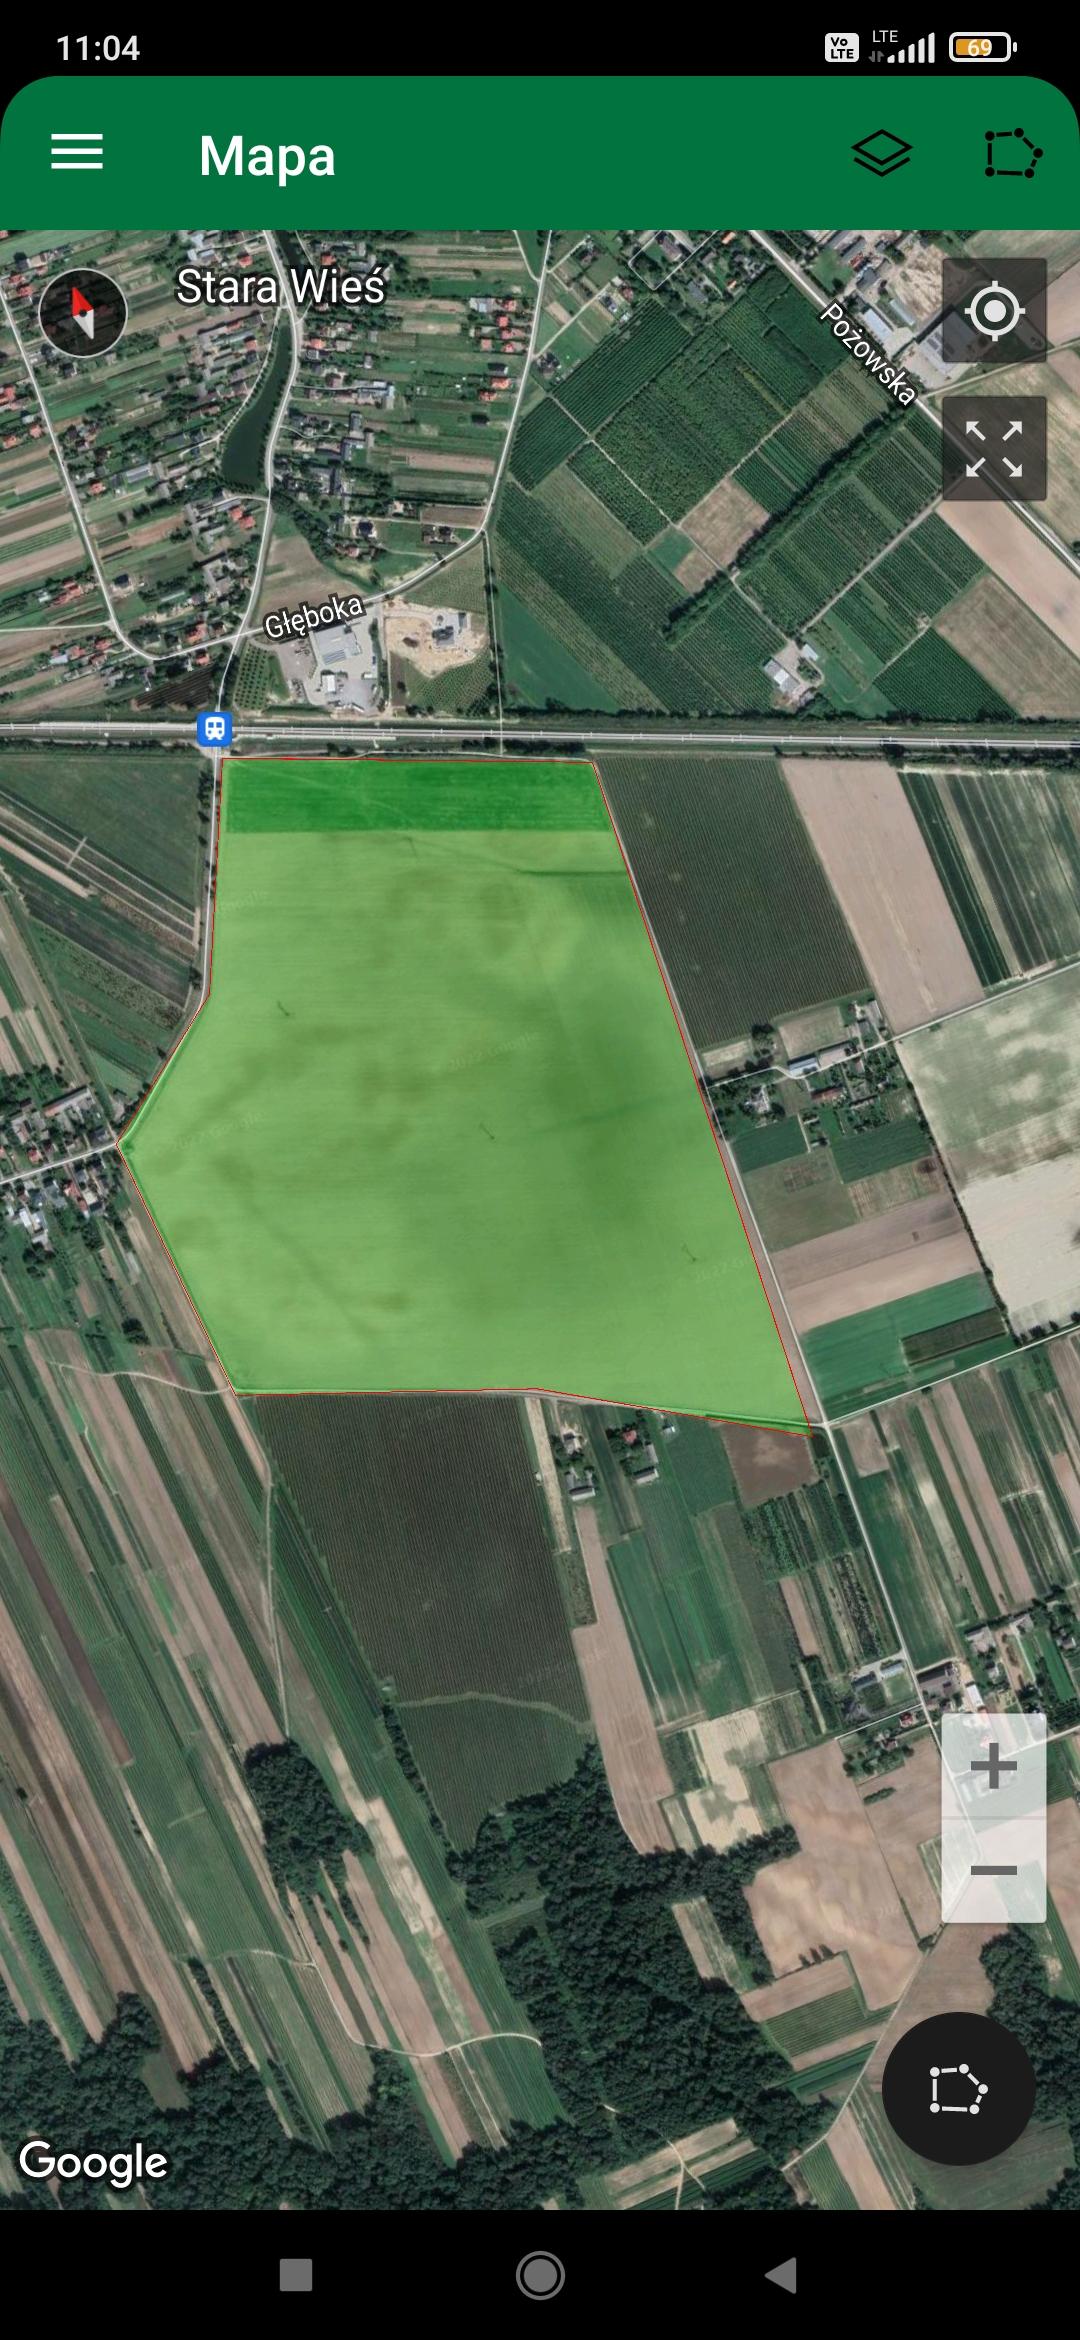
\includegraphics[width=0.8\textwidth]{grafika/nawigator_1.jpg}
			\caption{Granice pola oznaczone na mapie}
		\end{subfigure}%
		\begin{subfigure}{.5\textwidth}
			\centering
			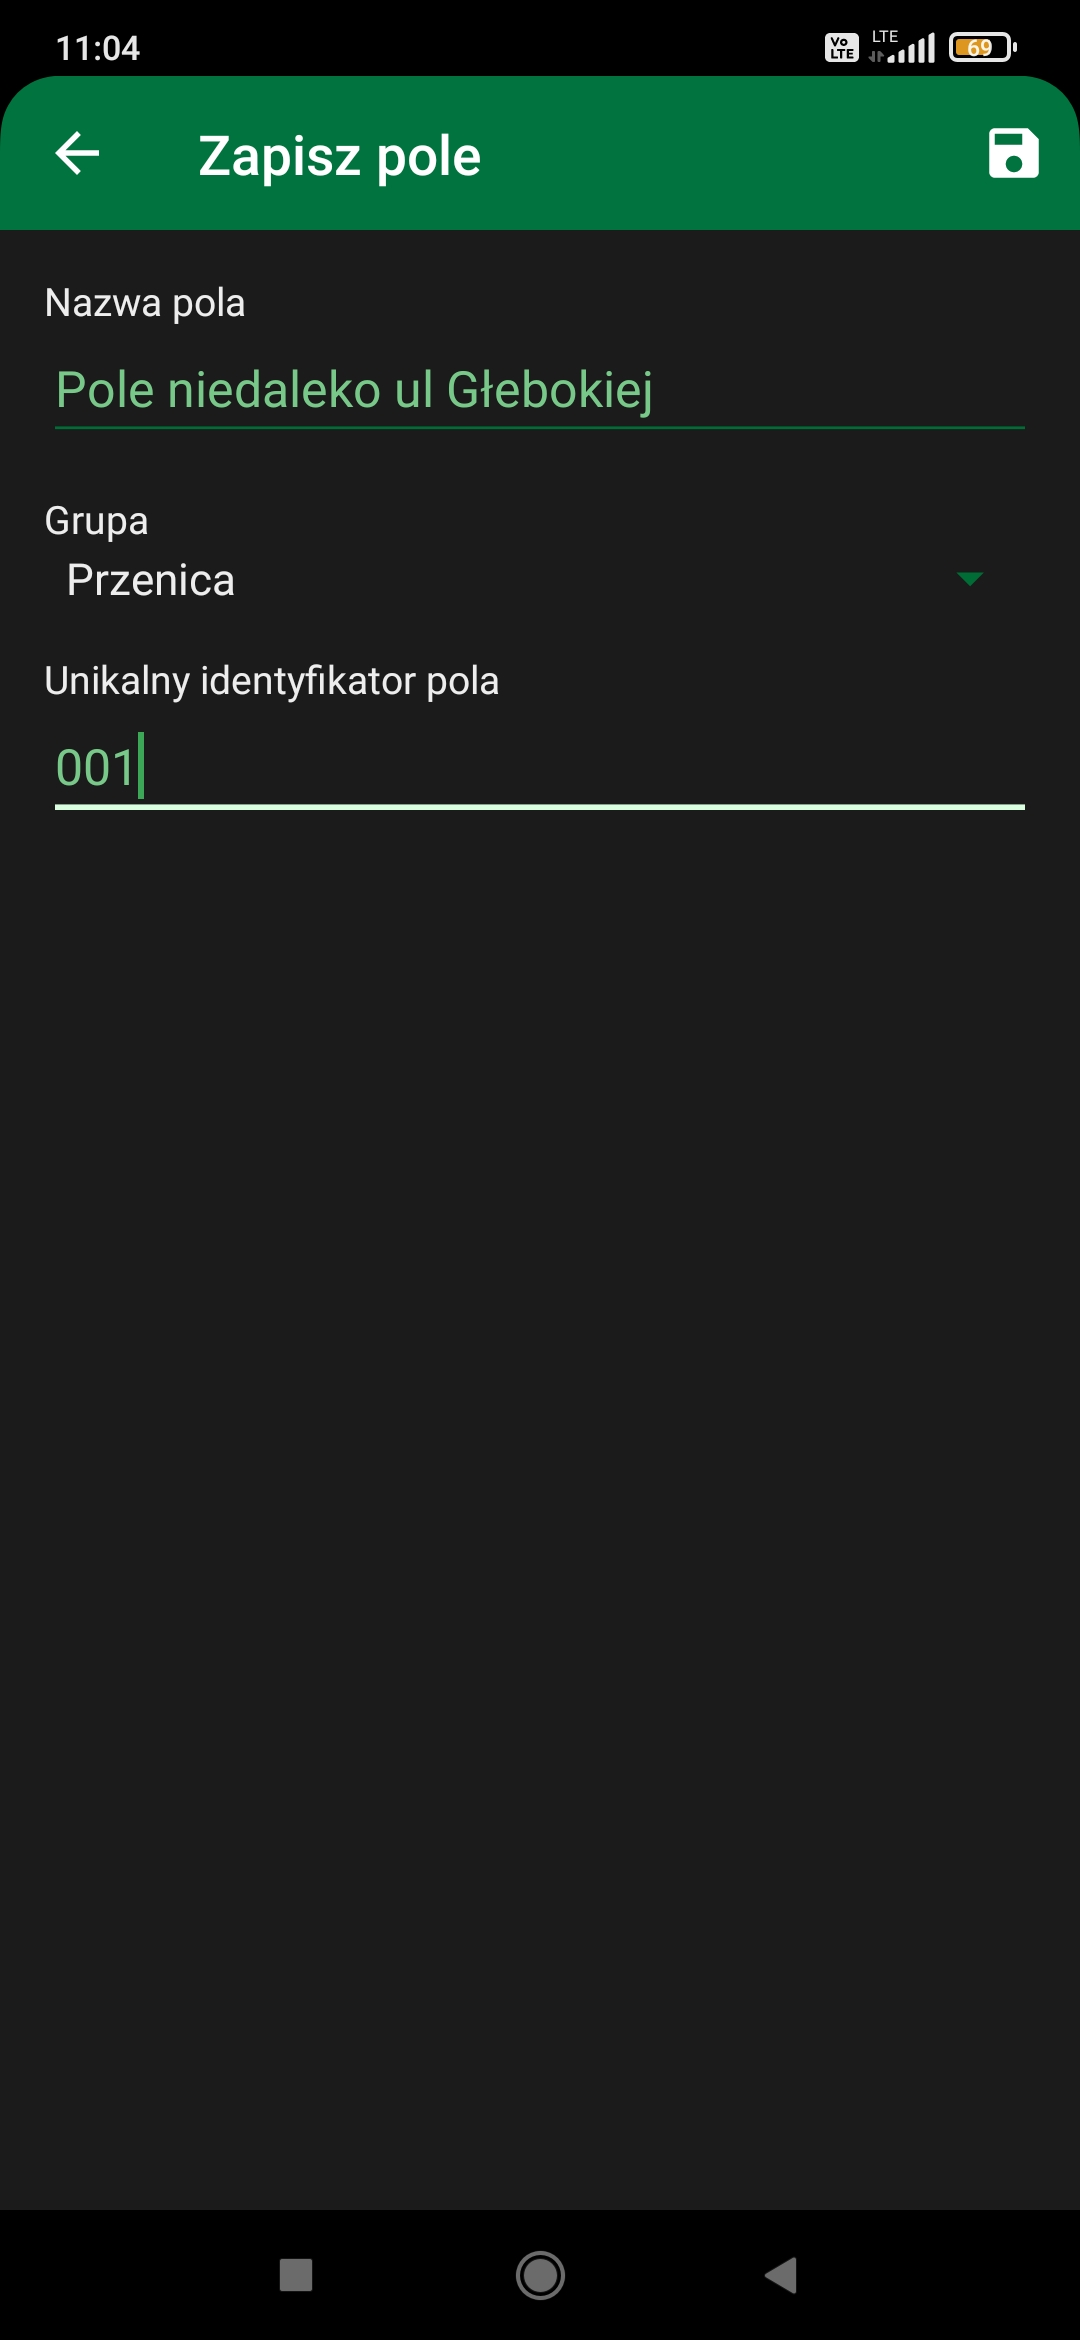
\includegraphics[width=0.8\textwidth]{grafika/nawigator_0.jpg}
			\caption{Zapisywanie informacji o polu}
		\end{subfigure}
		\caption{Zrzuty ekranu aplikacji "Nawigator polowy"}
	\end{figure}
	
	Innym przykładem dostępnych aplikacji dla rolników jest kalkulator rolniczy "Calcagro" \cite{ref7}. Sama aplikacja jest dosyć prosta w budowie jak i w obsłudze. W jej skład wchodzą proste kalkulatory obliczające: wagi odliczenia, ubytki na masie po suszeniu, wskaźniki wysiewu oraz stopy kapitalizacji. Interfejs użytkownika prezentuje się następująco (Rysunek 2.5). Jest to kolejna aplikacja, która posiada uproszczony oraz intuicyjny interfejs graficzny użytkownika.
	
	\begin{figure}[H]
		\centering
		\begin{subfigure}{.5\textwidth}
			\centering
			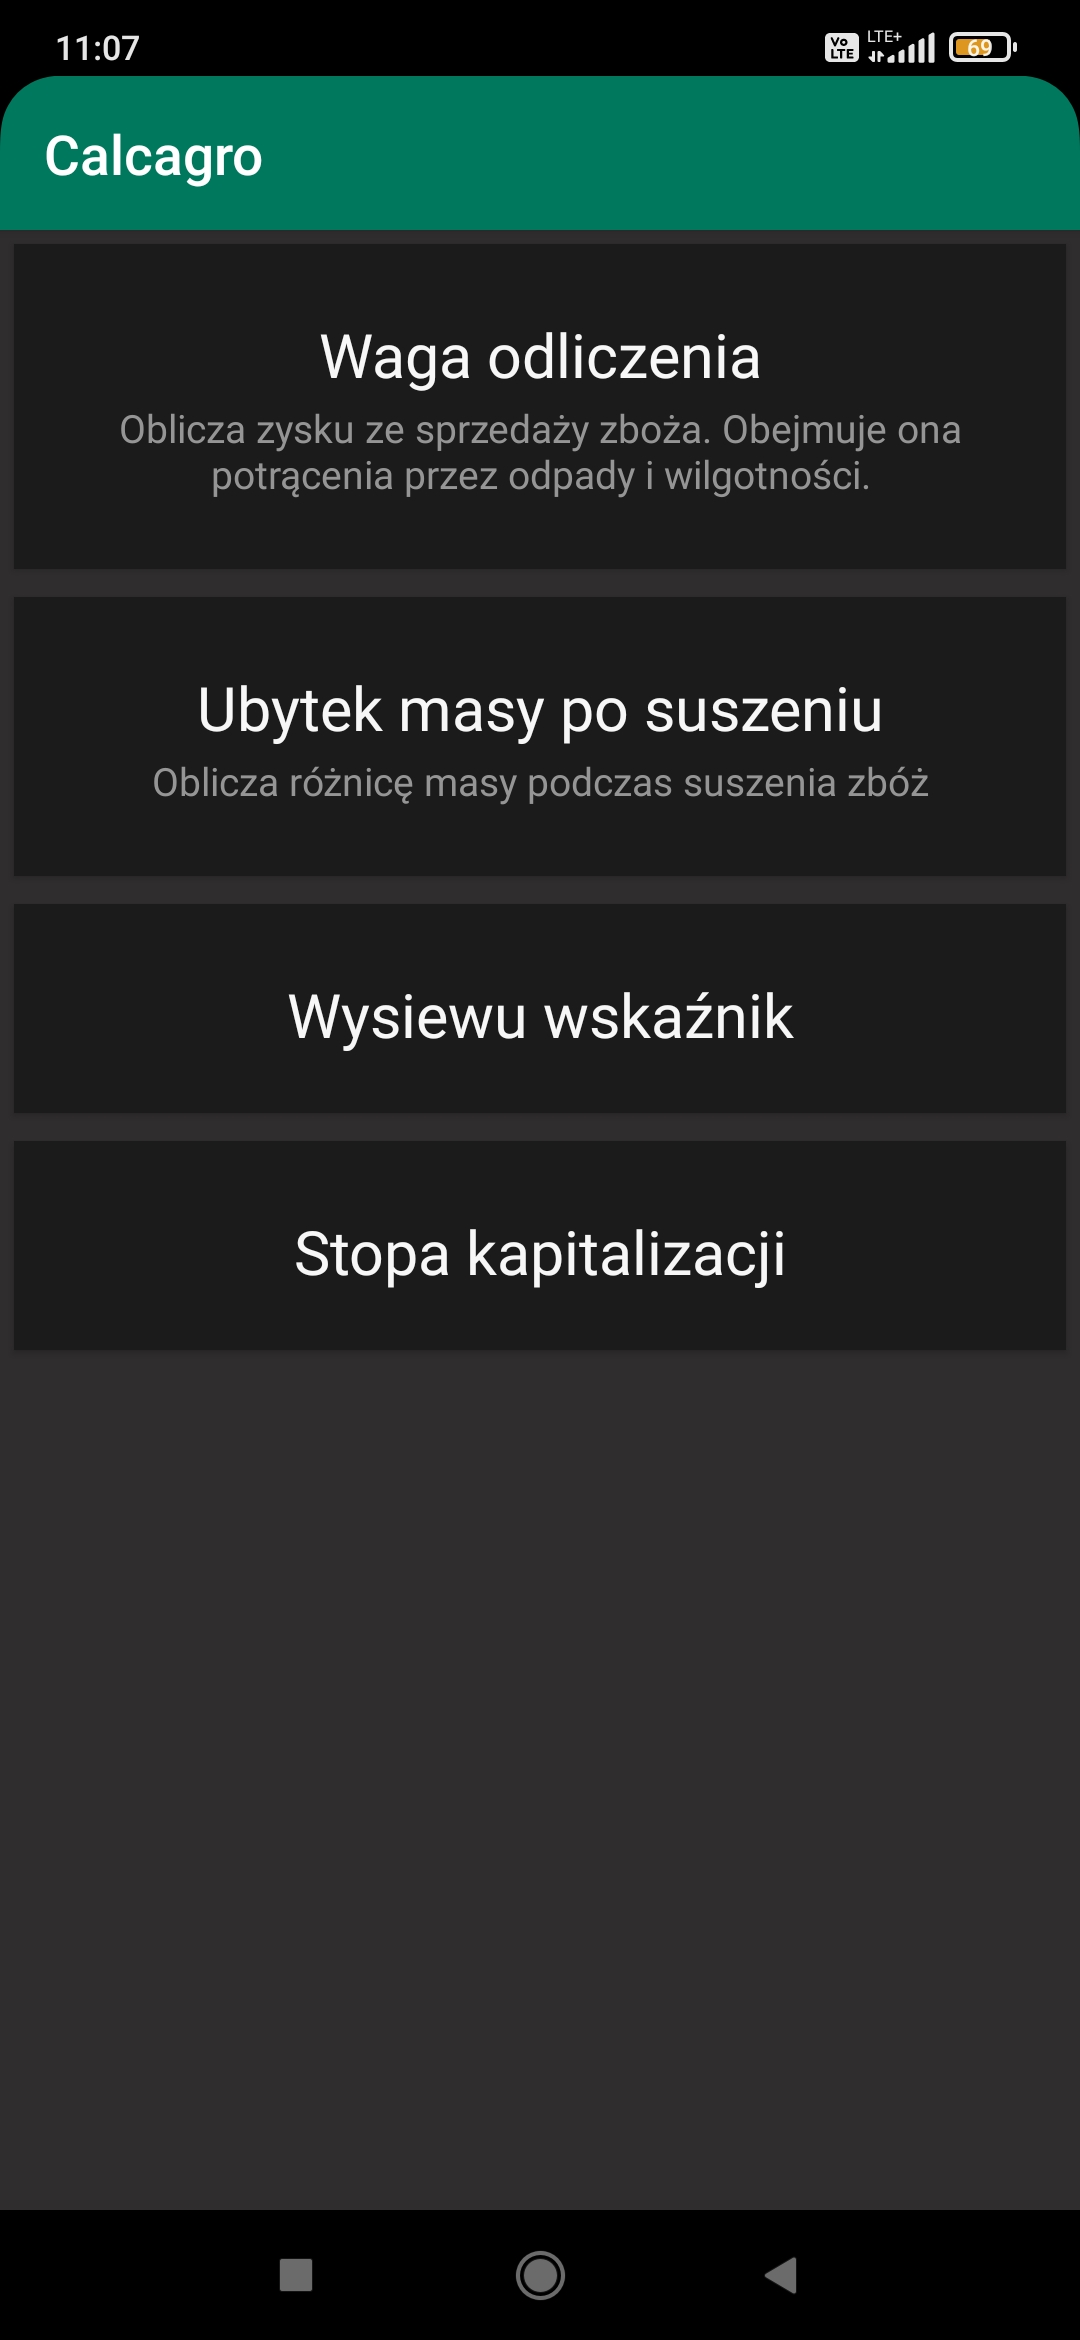
\includegraphics[width=0.8\textwidth]{grafika/calc_0.jpg}
			\caption{Dostępne kalkulatory}
		\end{subfigure}%
		\begin{subfigure}{.5\textwidth}
			\centering
			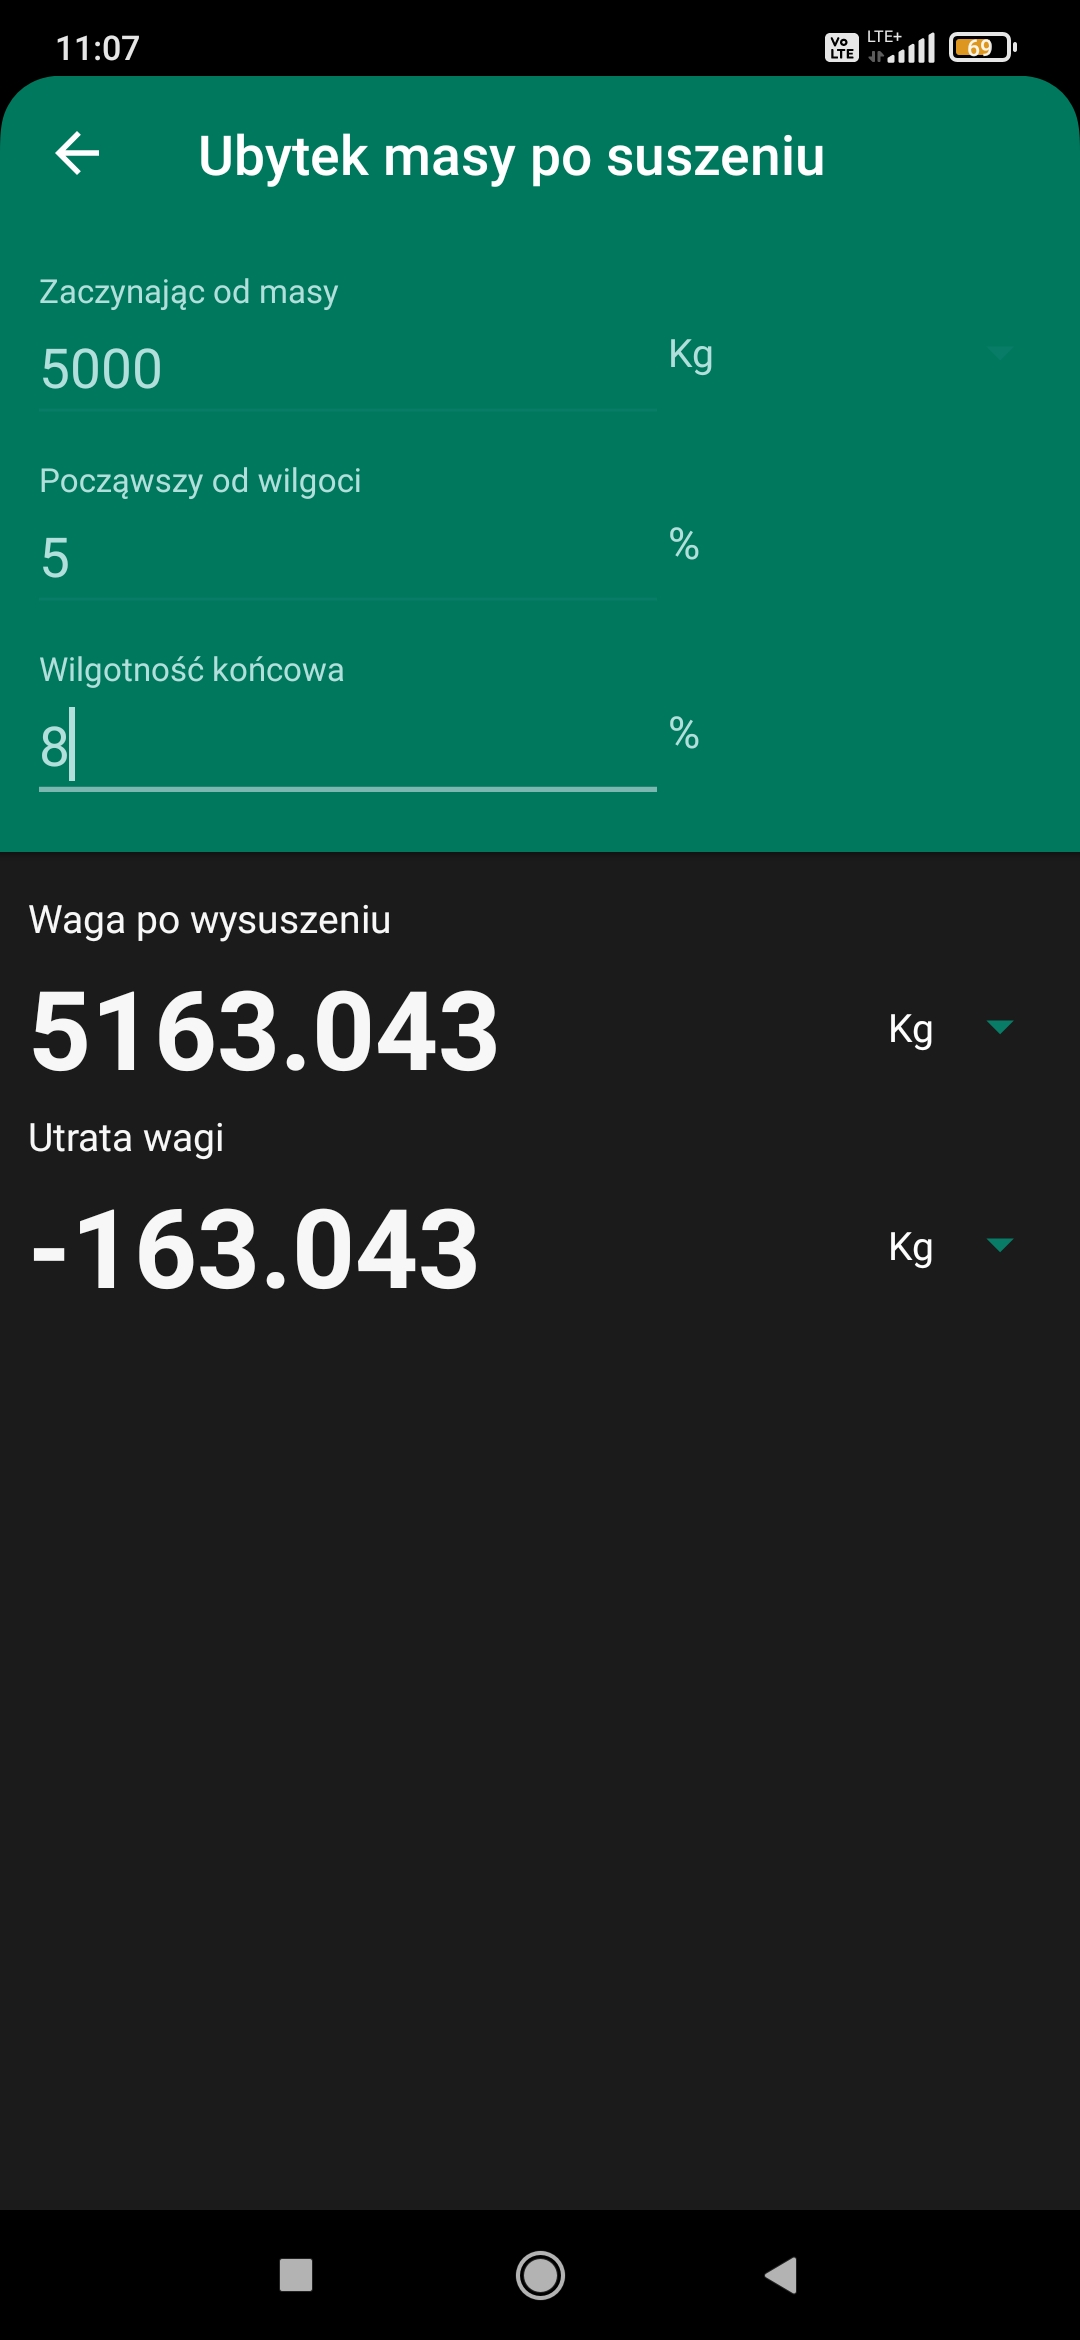
\includegraphics[width=0.8\textwidth]{grafika/calc_1.jpg}
			\caption{Obliczanie ubytku masy po suszeniu}
		\end{subfigure}
		\caption{Zrzuty ekranu aplikacji "Calcagro"}
	\end{figure}
	
	Ostatnim przykładem przedstawionym w tej pracy jest aplikacja "Agrobase" \cite{ref8}. Prostym interfejsem graficznym nie różni się od poprzednich aplikacji. Jej główną funkcjonalnością jest wyszukiwarka połączona z bazami danych chorób, szkodników, chwastów oraz środków ochrony roślin. W przypadku tej aplikacji wymagane jest pobranie bazy przy pierwszym użyciu danej funkcji, przy czym plusem jest możliwość wyboru danych dla danego państwa. Niestety aplikacja posiada kilka funkcjonalności tylko dla użytkowników premium. Wygląd aplikacji jest przedstawiony na Rysunku 2.6 .
	
	\begin{figure}[H]
		\centering
		\begin{subfigure}{.5\textwidth}
			\centering
			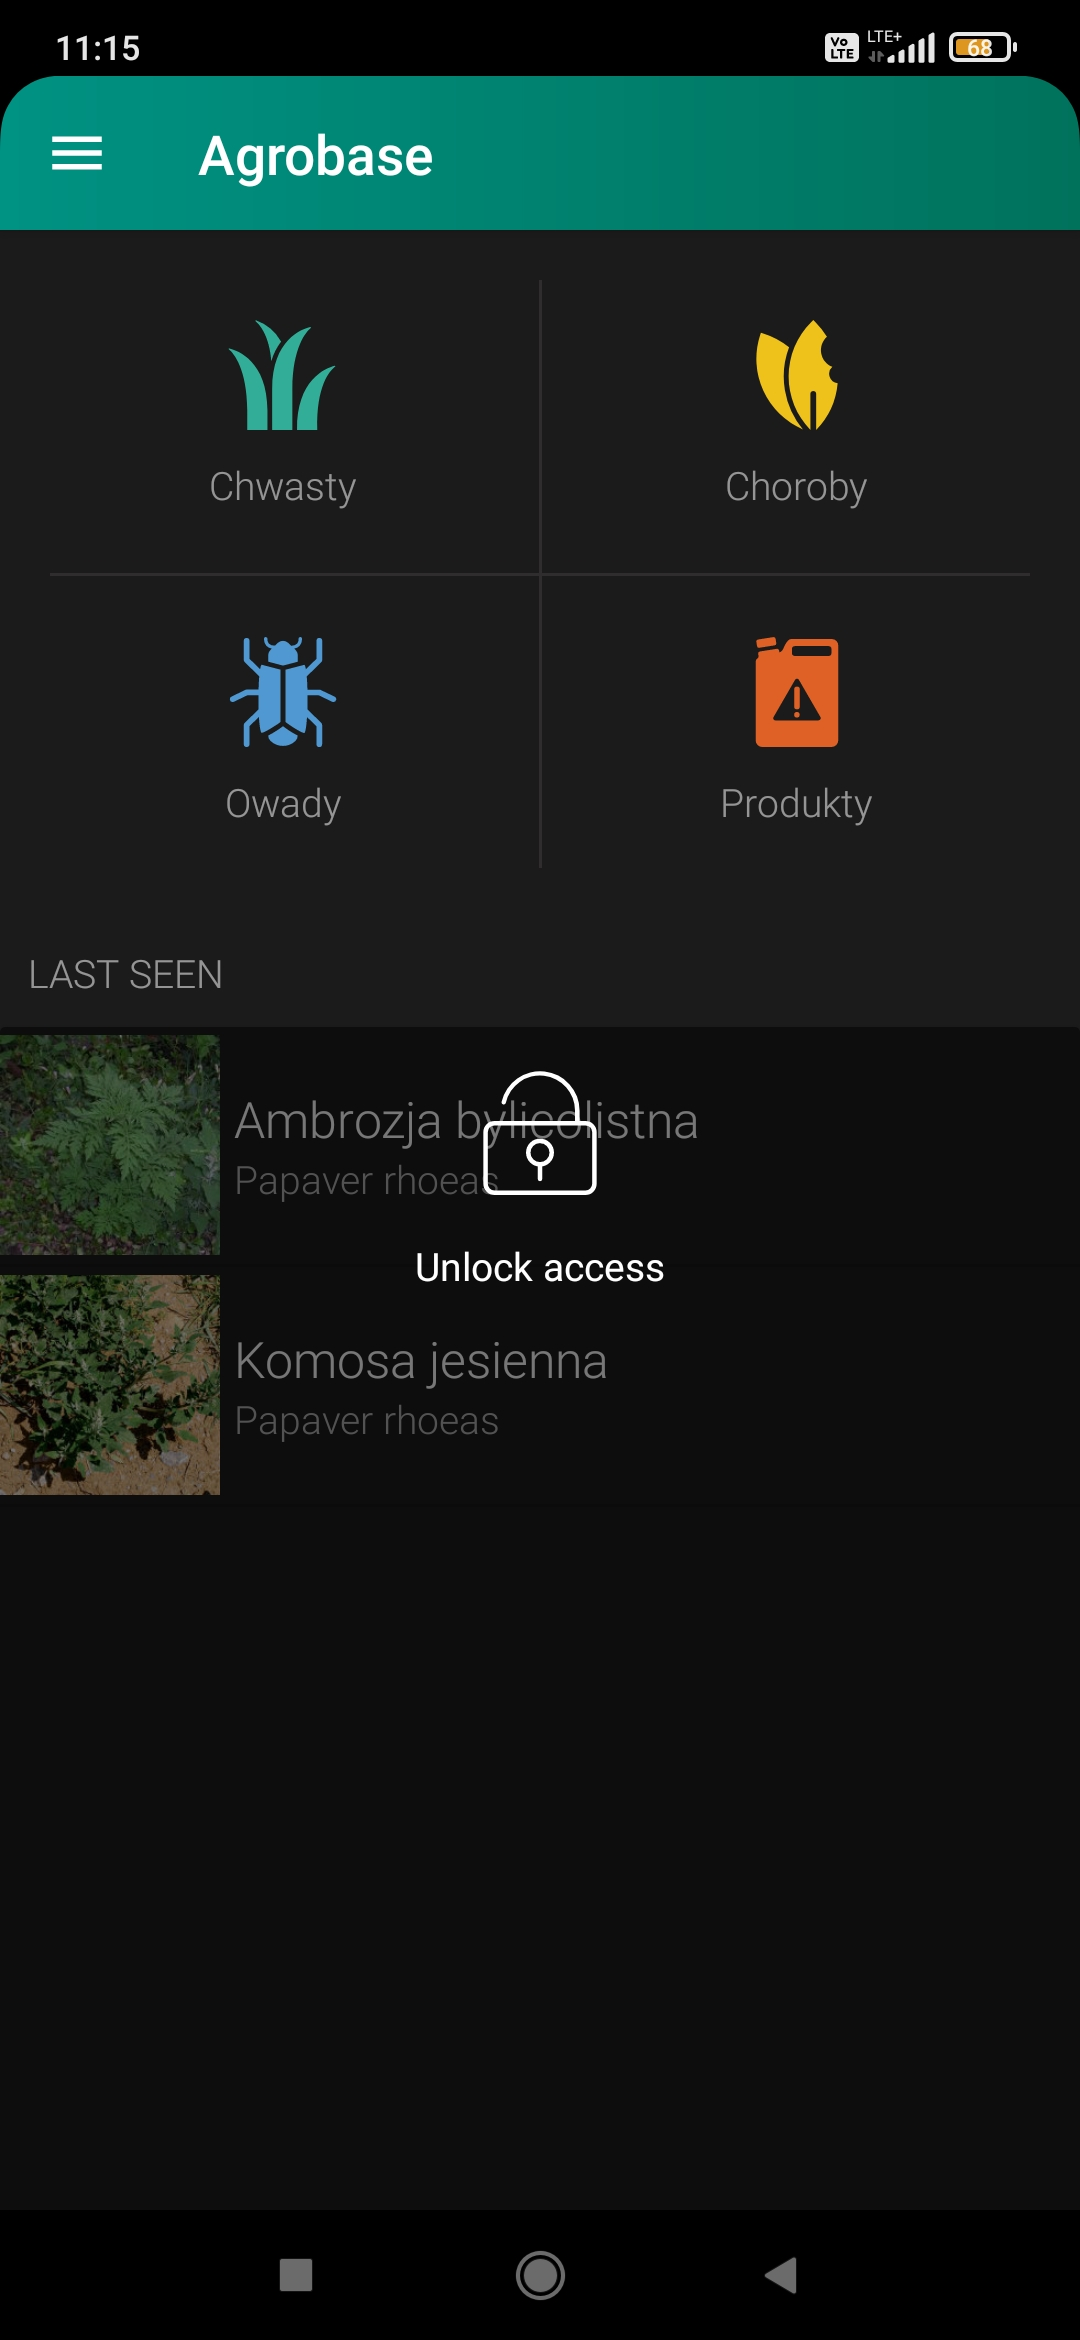
\includegraphics[width=0.8\textwidth]{grafika/db_0.jpg}
			\caption{Ekran główny}
		\end{subfigure}%
		\begin{subfigure}{.5\textwidth}
			\centering
			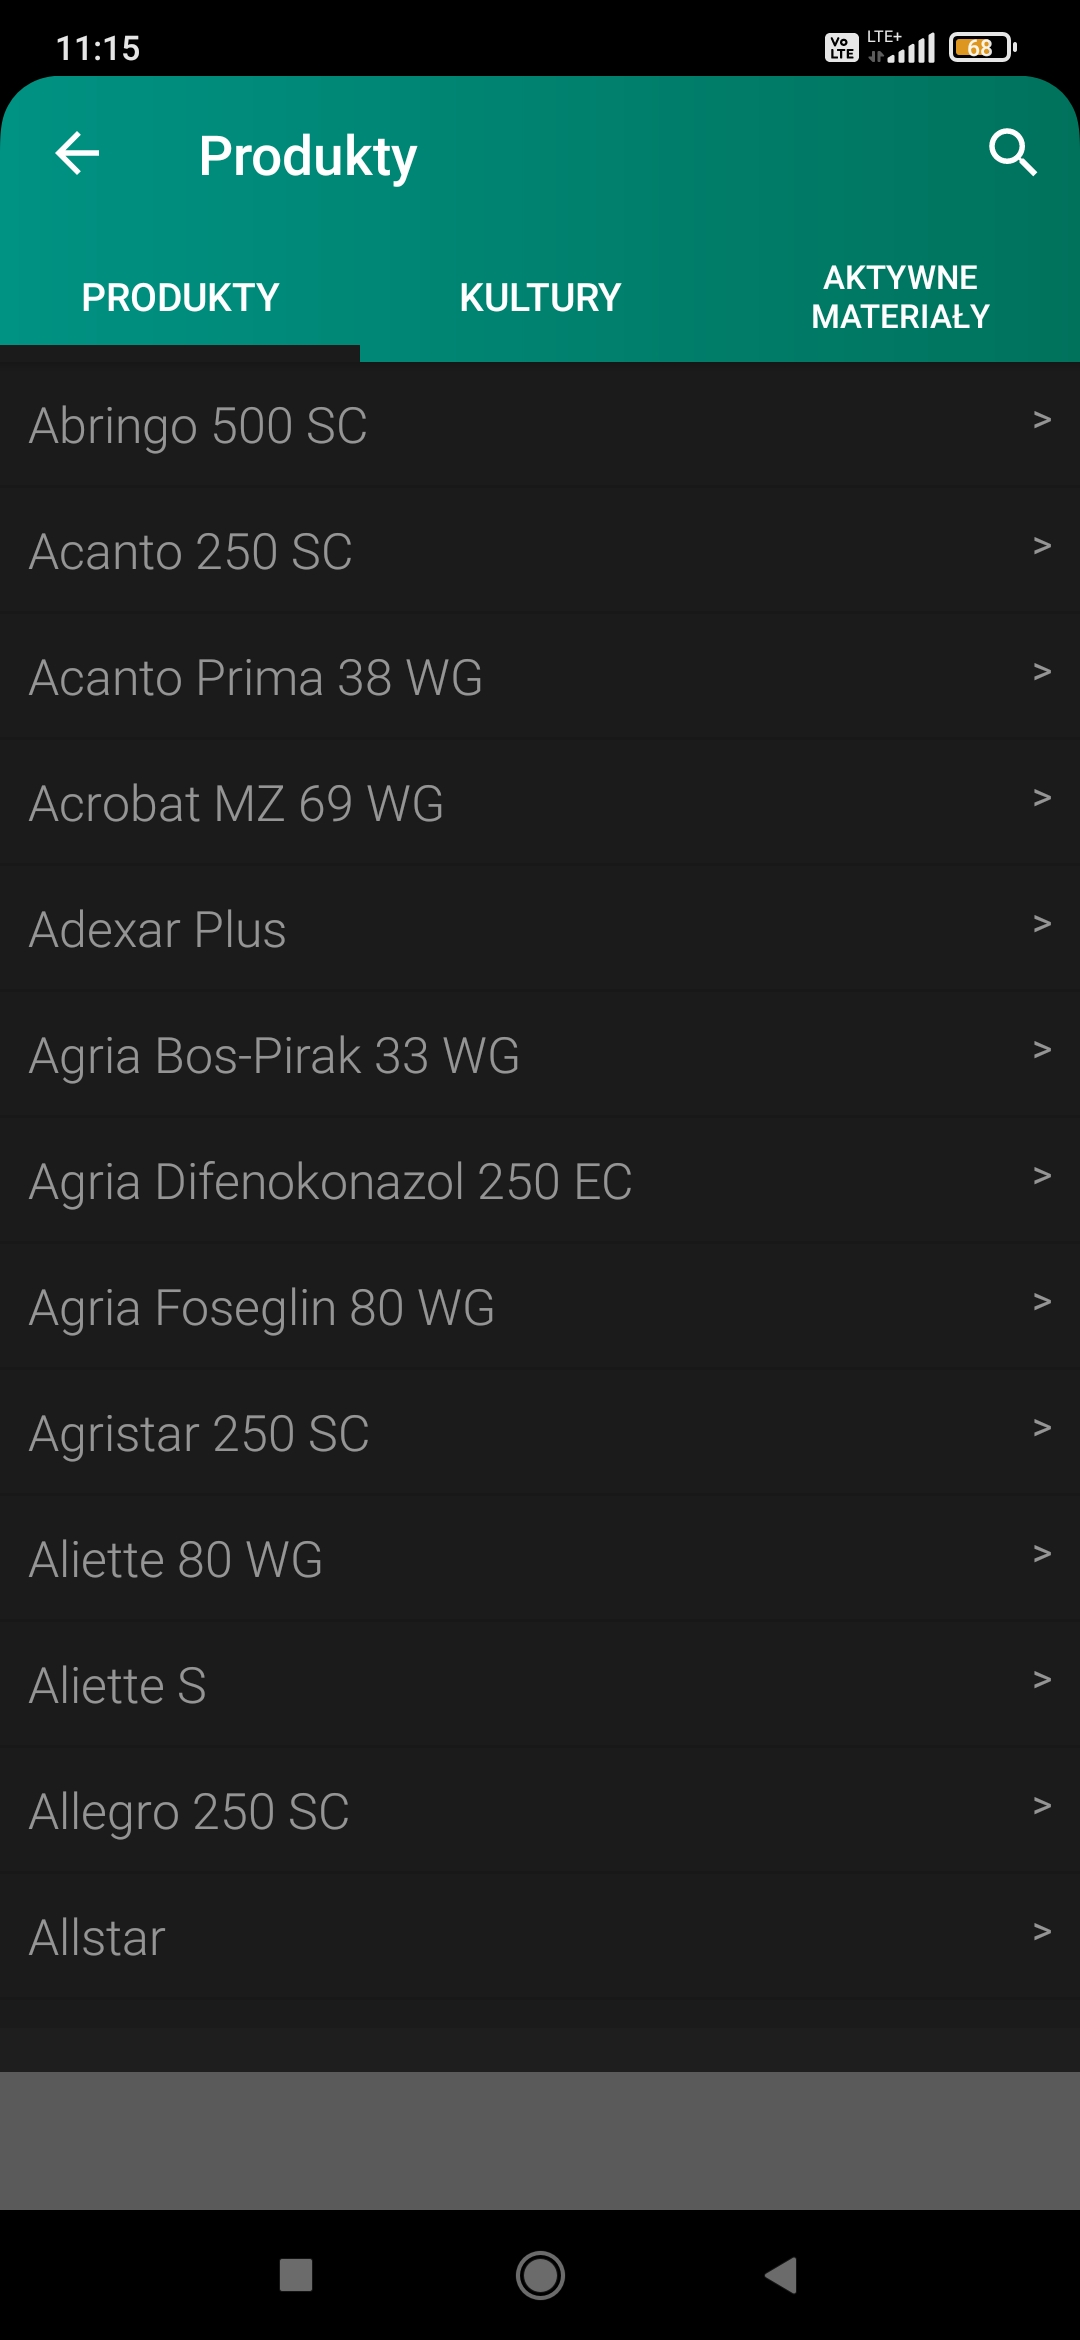
\includegraphics[width=0.8\textwidth]{grafika/db_2.jpg}
			\caption{Lista produktów}
		\end{subfigure}
		\caption{Zrzuty ekranu aplikacji "Agrobase"}
	\end{figure}

	Wymienione wyżej aplikacje posiadają szereg zalet takich jak prosty interfejs oraz intuicyjność użycia. Jeśli chodzi o wady to najbardziej zauważalnymi jest blokowanie niektórych funkcji za dodatkowymi opłatami. Aplikacje te posiadają po jednej głównej funkcjonalności, przez co użytkownik często musi pobierać wiele aplikacji od różnych twórców. Brakuje wśród nich rozwiązań, które posiadałyby wiele funkcji w jednej aplikacji, co zdecydowanie ułatwiło oraz zorganizowałoby pracę rolnika.
	
	\newpage
	\chapter{Agro4farm - aplikacja dla rolników}
	
	\section{O aplikacji}
	\ \ \ \
	W ramach praktyczniej części pracy zaprojektowana oraz zbudowana została mobilna aplikacja "Agro4Farm". Celem jej stworzenia było zorganizowanie oraz ułatwienie pracy dla osób pracujących na roli. Sama aplikacja została napisana z wykorzystaniem React Native w języku JavaScript przy użyciu platformy Expo.
	
	\section{React Native}
	\ \ \ \
	React Native jest otwarto-źródłowym frameworkiem bazującym na bibliotece React.js do języka JavaScript. Głównym celem stworzenia tego frameworku było utworzenie wygodnego środowiska dla programistów piszących aplikacje międzyplatformowe. Oprócz aplikacji na urządzenia mobilne, React Native pozwala tworzyć aplikacje na telewizory typu SmartTV oraz aplikacje wirtualnej rzeczywistości na urządzenia Oculus. Twórcą React Native jest jeden z gigantów rynku globalnego, czyli Meta.Inc dawniej nazywany Facebook. Jego pierwsza wersja wydana została w marcu 2015 roku. Framework jest na bieżąco aktualizowany, a jego kod źródłowy jest dostępny na GitHub \cite{ref9}.
	
	\newpage
	
	Framework React Native działa na bardzo podobnej zasadzie co React.js. Główną różnicą między nimi jest to, że React Native nie manipuluje DOM poprzez Virtual DOM, a działa w procesie w tle na urządzeniu końcowym, gdzie komunikuje się z platformą natywną. Tworzenie oraz stylizowanie elementów w React Native jest podobne do składni języków HTML i CSS.
	
	\begin{lstlisting}[caption=Kod przykłądowej aplikacji "Hello world" w React Native]
		import { StatusBar } from 'expo-status-bar';
		import { StyleSheet, Text, View } from 'react-native';
		
		export default function App() {
			return (
			<View style={styles.container}>
				<Text style={styles.text}>Hello world example!</Text>
				<StatusBar style="auto" />
			</View>
			);
		}
		
		const styles = StyleSheet.create({
			container: {
				flex: 1,
				backgroundColor: '#0D1317',
				alignItems: 'center',
				justifyContent: 'center',
			},
			text: {
				color: '#ffffff'
			},
		});
	\end{lstlisting}

	\begin{figure}[H]
		\centering
		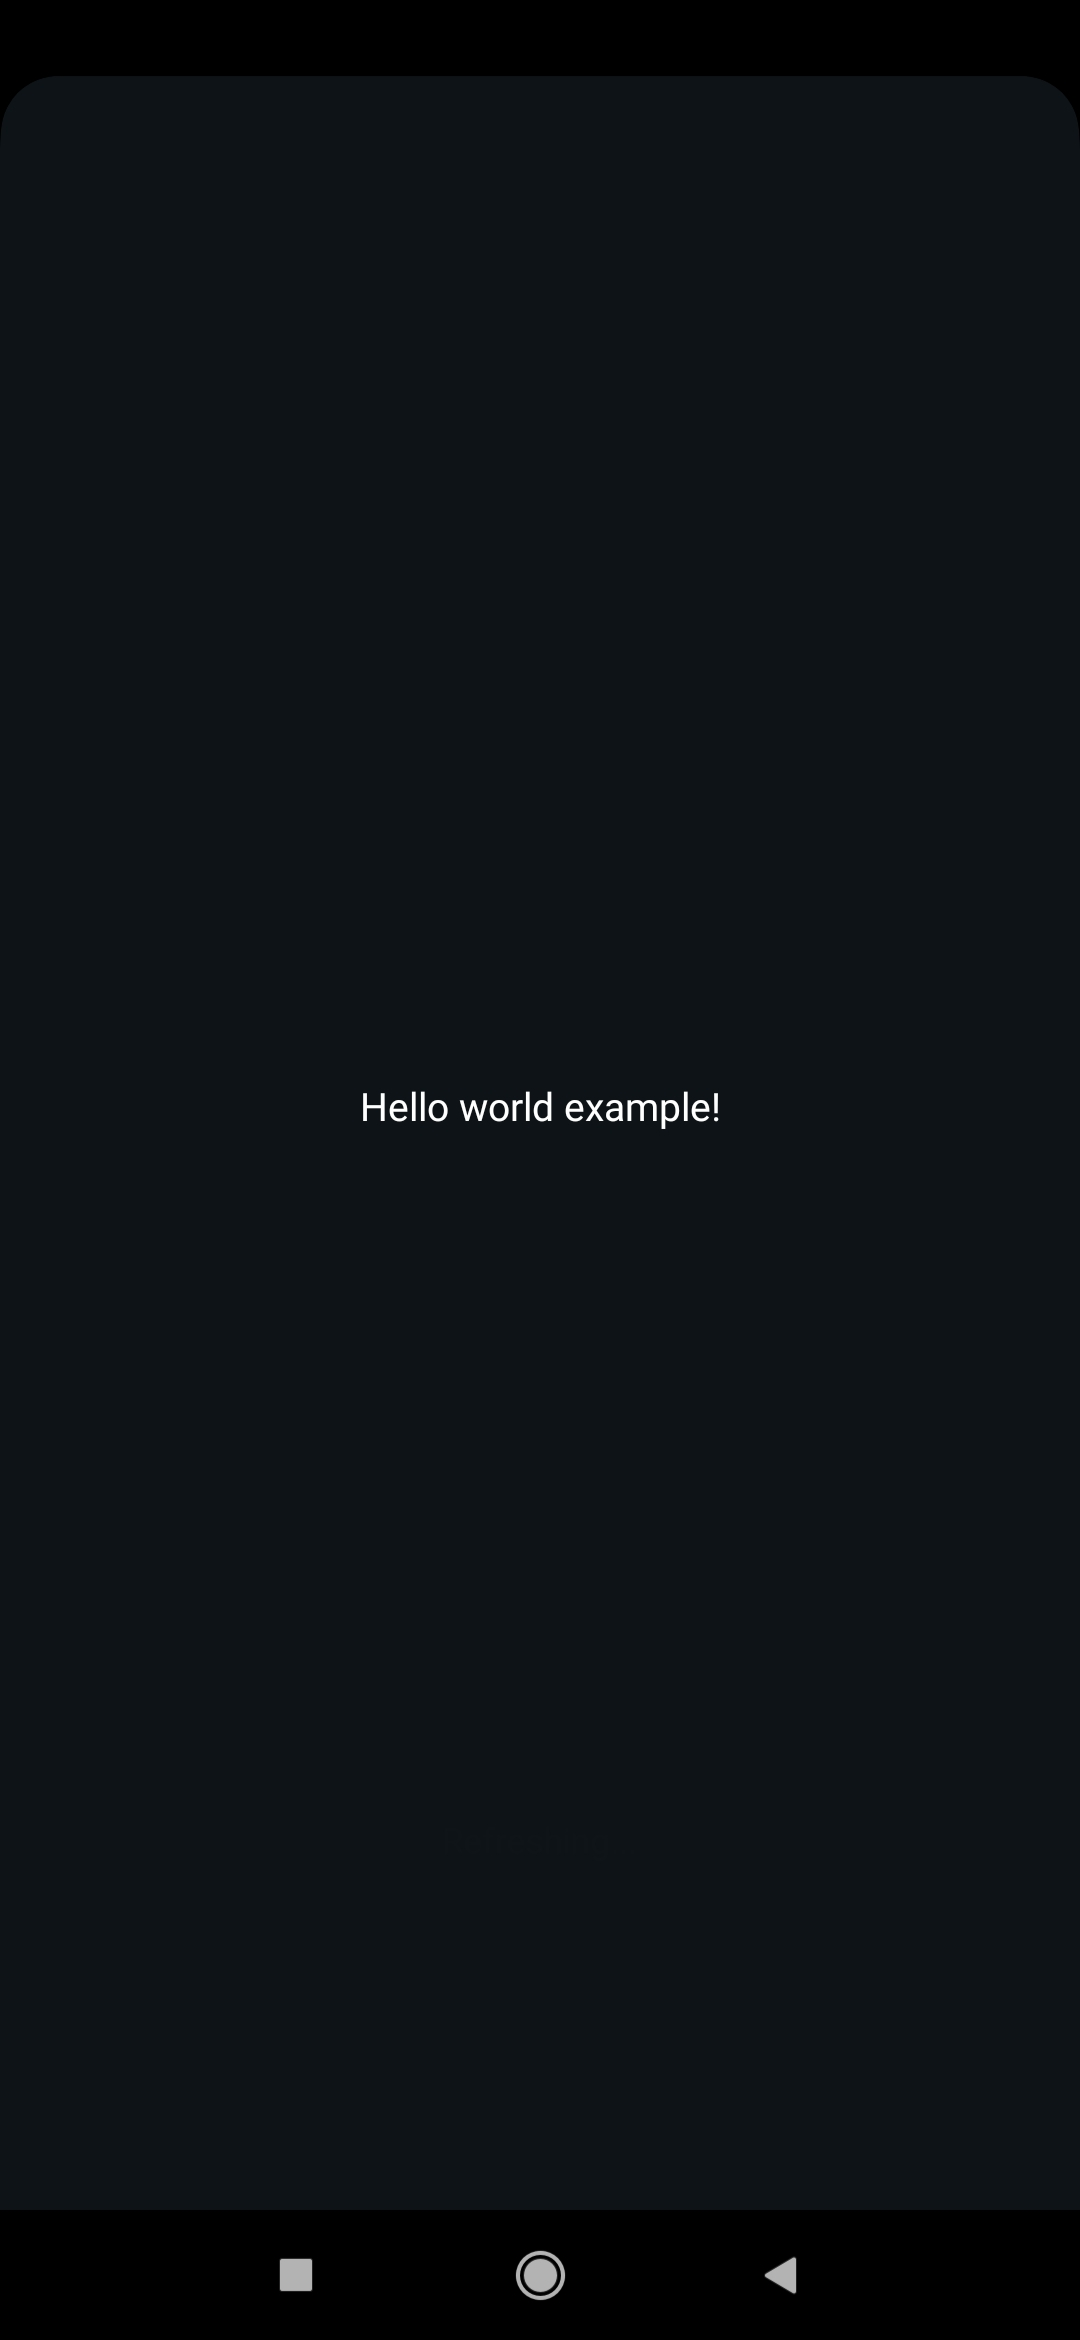
\includegraphics[width=0.5\textwidth]{grafika/hello_world.jpg}
		\caption{Przykładowa aplikacja mobilna "Hello world!"}
	\end{figure}

	Tak jak zostało to przedstawione w Listingu 3.1, główną częścią aplikacji jest funkcja "App", w której to zwracany jest główny widok. Komponenty takie jak View, Text, StyleSheet czy StatusBar muszą być wcześniej zaimportowane z konkretnych bibliotek. Poszczególne komponenty posiadają swoje atrybuty. W przykładzie można zauważyć użycie atrybutu "style", którego wartości przekazywane są w postaci zmiennej "styles". Efekt końcowy aplikacji widać na załączonym Rysunku 3.1.
	
	\subsection{Expo}
	\ \ \ \
	Expo to otwarta platforma do tworzenia natywnych aplikacji przy użyciu React Native. Expo pozwala na tworzenie aplikacji mobilnych na urządzenia z systemem Android i iOS oraz na platformy webowe. Narzędzie to stworzono w celu szybkiego rozpoczęcia pracy oraz jej ułatwienia. Po zainstalowaniu odpowiednich narzędzi na urządzeniu, użytkownik poprzez konsole może zainstalować Expo, a następnie stworzyć nowy projekt. Dodatkowo Expo daje możliwość prostego uruchamiania projektów w aplikacji Expo Go, dzięki której użytkownik jest w stanie debugować aplikację oraz korzystać z opcji przeładowanie na gorąco (ang: Hot reload).
	
	\section{Funkcjonalności}
	\ \ \ \
	Aplikacja Agro4Farm składa się z pięciu głównych funkcjonalności. Ideą jej było zebranie najbardziej przydatnych opcji w jednym miejscu w celu uproszczenia oraz organizacji pracy użytkownika. Funkcjami, które zawierają się w aplikacji są:
	\begin{description}
		\item[Pogoda] - aktualna prognoza pogody.
		\item[Kalkulator wysiewu zbóż] - prosty kalkulator obliczający wartości wysiewu zbóż wraz z informacjami na temat danych zbóż.
		\item[Notatki] - funkcja tworzenia oraz zapisywania notatek.
		\item[Baza środków ochrony roślin] - baza danych z wyszukiwarką chorób, upraw oraz środków ochrony roślin.
		\item[Przewidywanie terminów pracy i nawożenia] - funkcja przewidująca dogodne terminy pracy na podstawie pogody.
	\end{description}
	
	\newpage
	
	\subsection{Pogoda}
	\ \ \ \
		Jednym z najważniejszych czynników określającym to, czy rolnik jest w stanie wykonywać swoje obowiązki jest pogoda. To właśnie od warunków atmosferycznych takich jak ilość opadów, wilgotność czy siła wiatru zależy czy rolnik będzie w stanie wykonywać swoją pracę. Dlatego właśnie pierwszą funkcją aplikacji jest prognoza pogody. Jest to dosyć prosta funkcjonalność pozwalająca na sprawdzanie aktualnej prognozy pogody. Funkcja ta używa darmowego ogólnodostępnego interfejsu OpenWeather API, który pozwala na wykonywanie prostych zapytań w celu uzyskania aktualnych informacji pogodowych. 
		
		Wymieniony wyżej interfejs programowania aplikacji inaczej API (ang: Application Programming Interface) to interfejs pozwalający na komunikację z aplikacjami oraz serwerami. Pozwala on między innymi na uzyskiwanie danych poprzez wysyłanie zapytań (Rysunek 3.2) \cite{ref13}. 
	
	\begin{figure}[H]
		\centering
		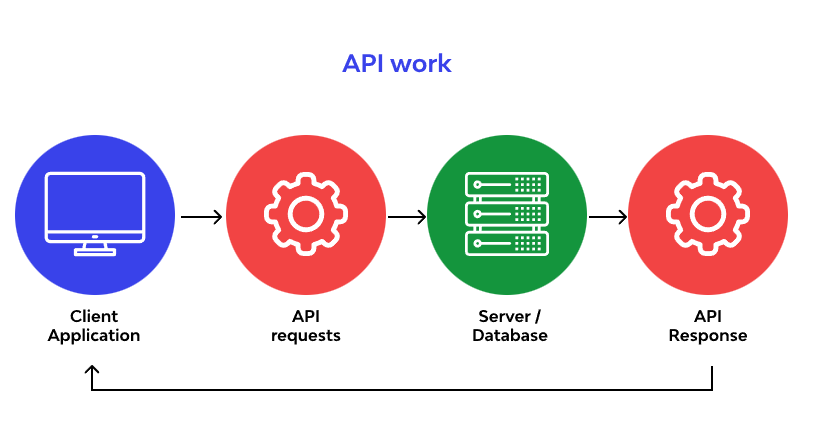
\includegraphics[width=0.9\textwidth]{grafika/api.png}
		\caption{Schemat działania interfejsu API}
	\end{figure}

	Po wykonaniu odpowiedniego zapytania, OpenWeather API zwraca użytkownikowi obiekt w formacie JSON z informacjami o pogodzie. Informacje które z takiego obiektu jesteśmy w stanie odczytać to: opis pogody, koordynaty lokacji, wiatr, wilgotność, wschód i zachód słońca oraz wiele więcej.
	
	\newpage
	
	\begin{lstlisting}[caption=Przykładowa odpowiedź z OpenWeather API]
		{
			"coord": {
				"lon": -122.08,
				"lat": 37.39
			},
			"weather": [
			{
				"id": 800,
				"main": "Clear",
				"description": "clear sky",
				"icon": "01d"
			}
			],
			"main": {
				"temp": 282.55,
				"feels_like": 281.86,
				"temp_min": 280.37,
				"temp_max": 284.26,
				"pressure": 1023,
				"humidity": 100
			},
			"wind": {
				"speed": 1.5,
				"deg": 350
			},
			"sys": {
				"type": 1,
				"id": 5122,
				"message": 0.0139,
				"country": "US",
				"sunrise": 1560343627,
				"sunset": 1560396563
			},
			"timezone": -25200,
			"id": 420006353,
			"name": "Mountain View",
			"cod": 200
		} 
	\end{lstlisting}

	Aby otrzymać odpowiedź podobną do odpowiedzi przedstawionej w Listingu 3.2 należy najpierw wykonać odpowiednie zapytanie, które może wyglądać następująco (Listing 3.3).
	
	\begin{lstlisting}[caption=Przykład zapytania do OpenWeather API]
		const api = {
			link: "https://api.openweathermap.org/data/2.5/weather?",
			key: "cba123defg0987qwerte2f238"
		}
	
		async function fetchWeather() {
			let { status } = await Location.requestForegroundPermissionsAsync()
			const location = await Location.getCurrentPositionAsync()
			const { latitude, longitude } = location.coords
			
			const URL = `${api.link}lat=${latitude}&lon=${longitude}&lang=pl&units=metric&appid=${api.key}`
			
			const weatherFetch = await fetch(URL)
			const result = await weatherFetch.json()
			if (weatherFetch.ok) {
				setWeather(result)
			} else {
				setErrorMsg(result.message)
			}
		}
	\end{lstlisting}
	
	W powyższym zapytaniu w linijce 11 tworzony jest adres URL zapytania. W nim podawane są współrzędne geograficzne aktualnej lokalizacji, język w jakim dane zostaną zwrócone, typ jednostek oraz klucz API. Klucz API jest unikalny dla twórcy, a jego generowanie jest możliwe na stronie OpenWeather API. Jeśli chodzi o lokalizację, wartości wysokości oraz szerokości geograficznej są pobierane za pomocą funkcji lokalizacji w telefonie. 
	
	\newpage
	
	W przypadku otrzymania poprawnej odpowiedzi, otrzymane wartości zapisywane są pod określoną zmienną, a w przeciwnym wypadku ustawiana jest odpowiednia wiadomość z błędem. Gotowa funkcjonalność prezentuje się następująco na Rysunku 3.3
	
	\begin{figure}[H]
		\centering
		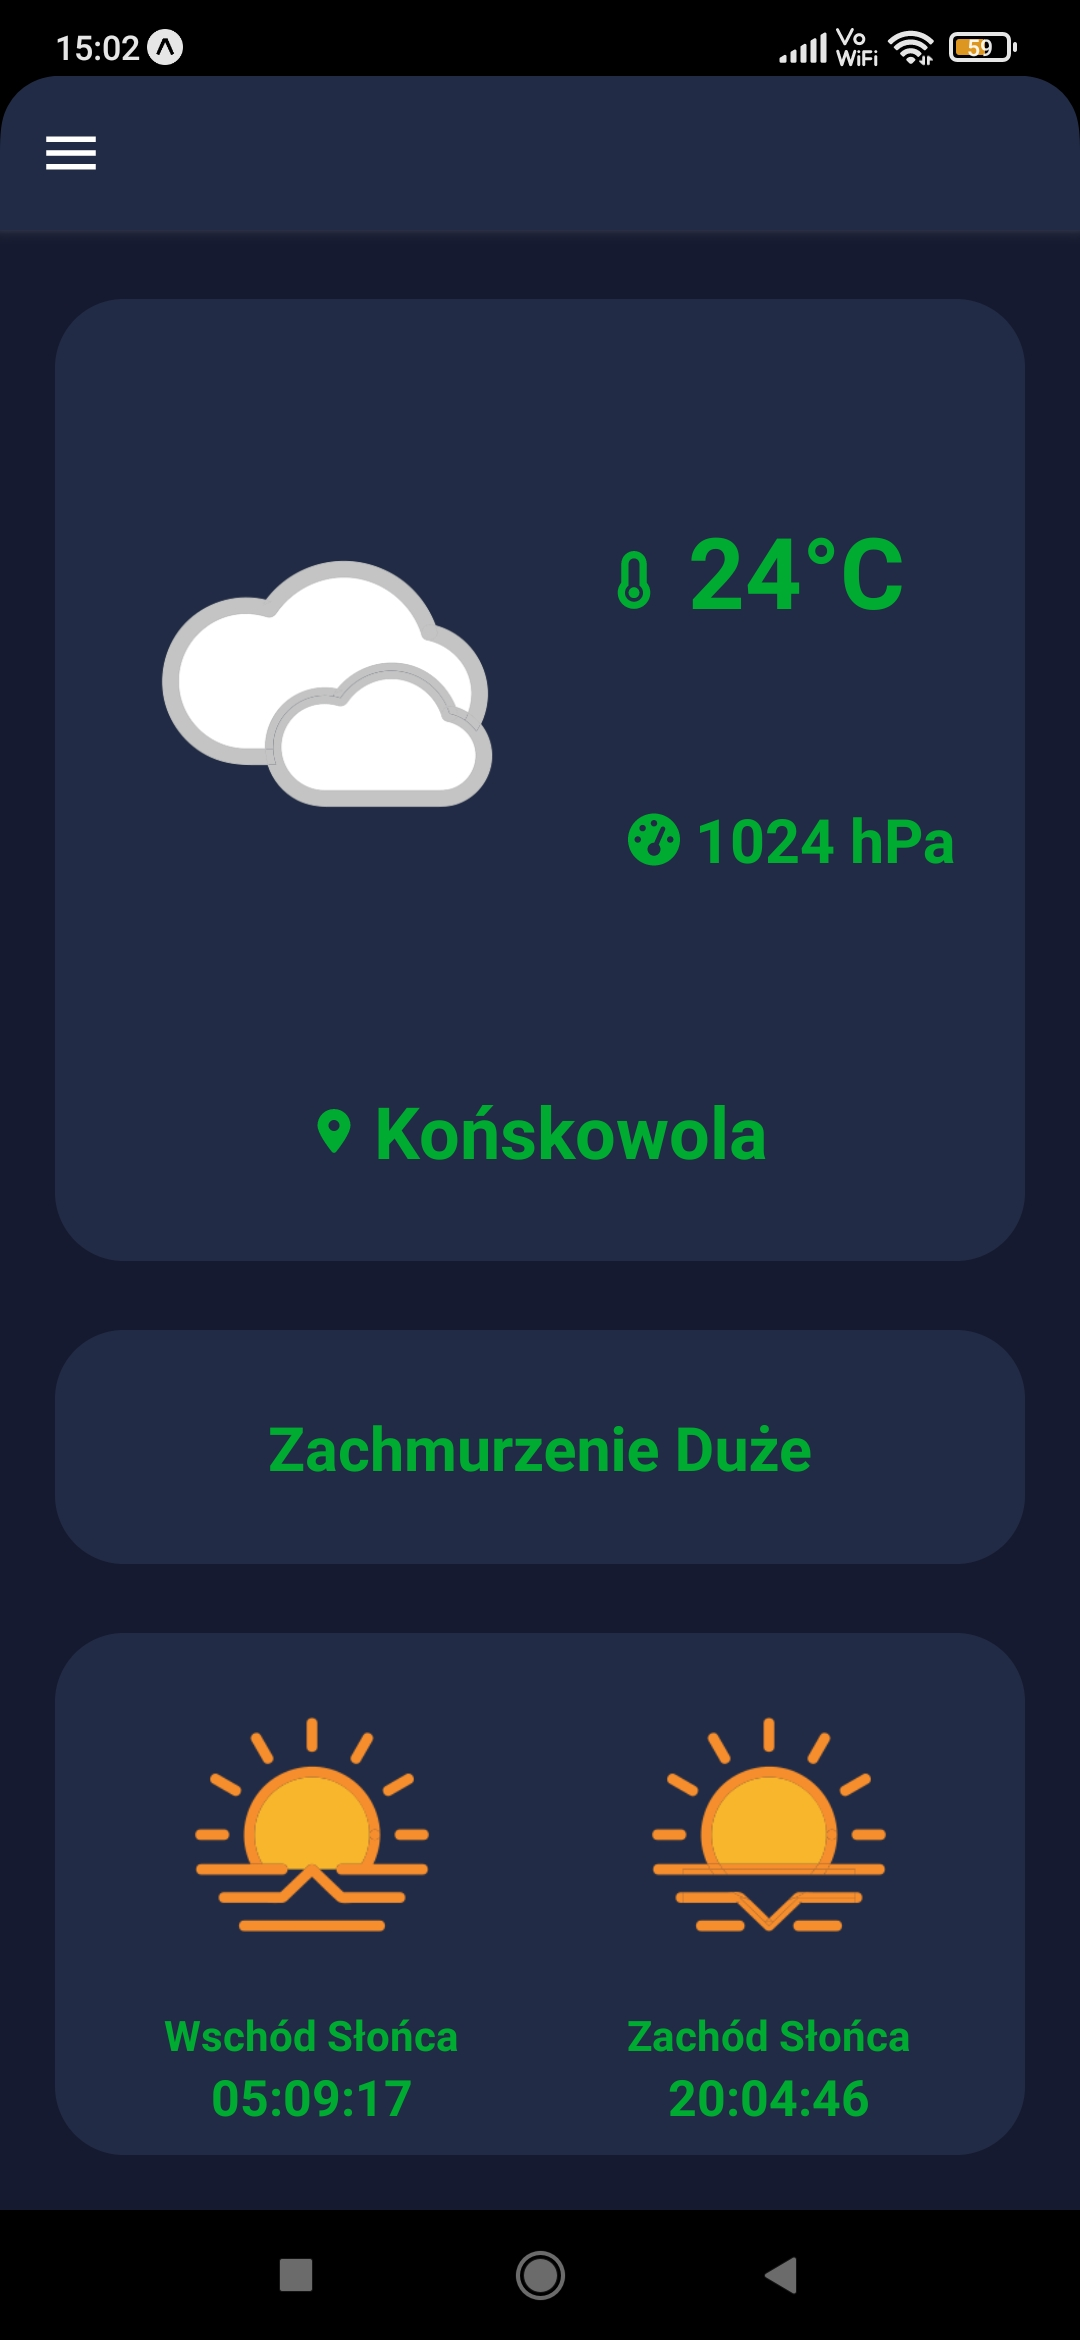
\includegraphics[width=0.55\textwidth]{grafika/pogoda.jpg}
		\caption{Zrzut ekranu funkcji "Pogoda"}
	\end{figure}
	
	\subsection{Notatki}
	\ \ \ \
		Kolejną możliwością aplikacji Agro4Farm jest tworzenie notatek. Jest to dosyć prosta funkcjonalność, której głównym celem jest przechowywanie najważniejszych dla użytkownika informacji w pamięci telefonu. Funkcja ta do działania wykorzystuje bibliotekę "AsyncStorageLib", czyli asynchroniczny system przetrzymywania danych bazujący na kluczach i ich wartościach. Funkcja przy tworzeniu nowej notatki zapisuje tytuł oraz jej treść, co pozwala później na łatwe wyszukiwanie zapisanych notatek (Rysunek 3.4a). Wszystkie notatki natomiast wyświetlane są za pomocą przewijanej listy (Rysunek 3.4b).
		
	\begin{figure}[H]
		\centering
		\begin{subfigure}{.5\textwidth}
			\centering
			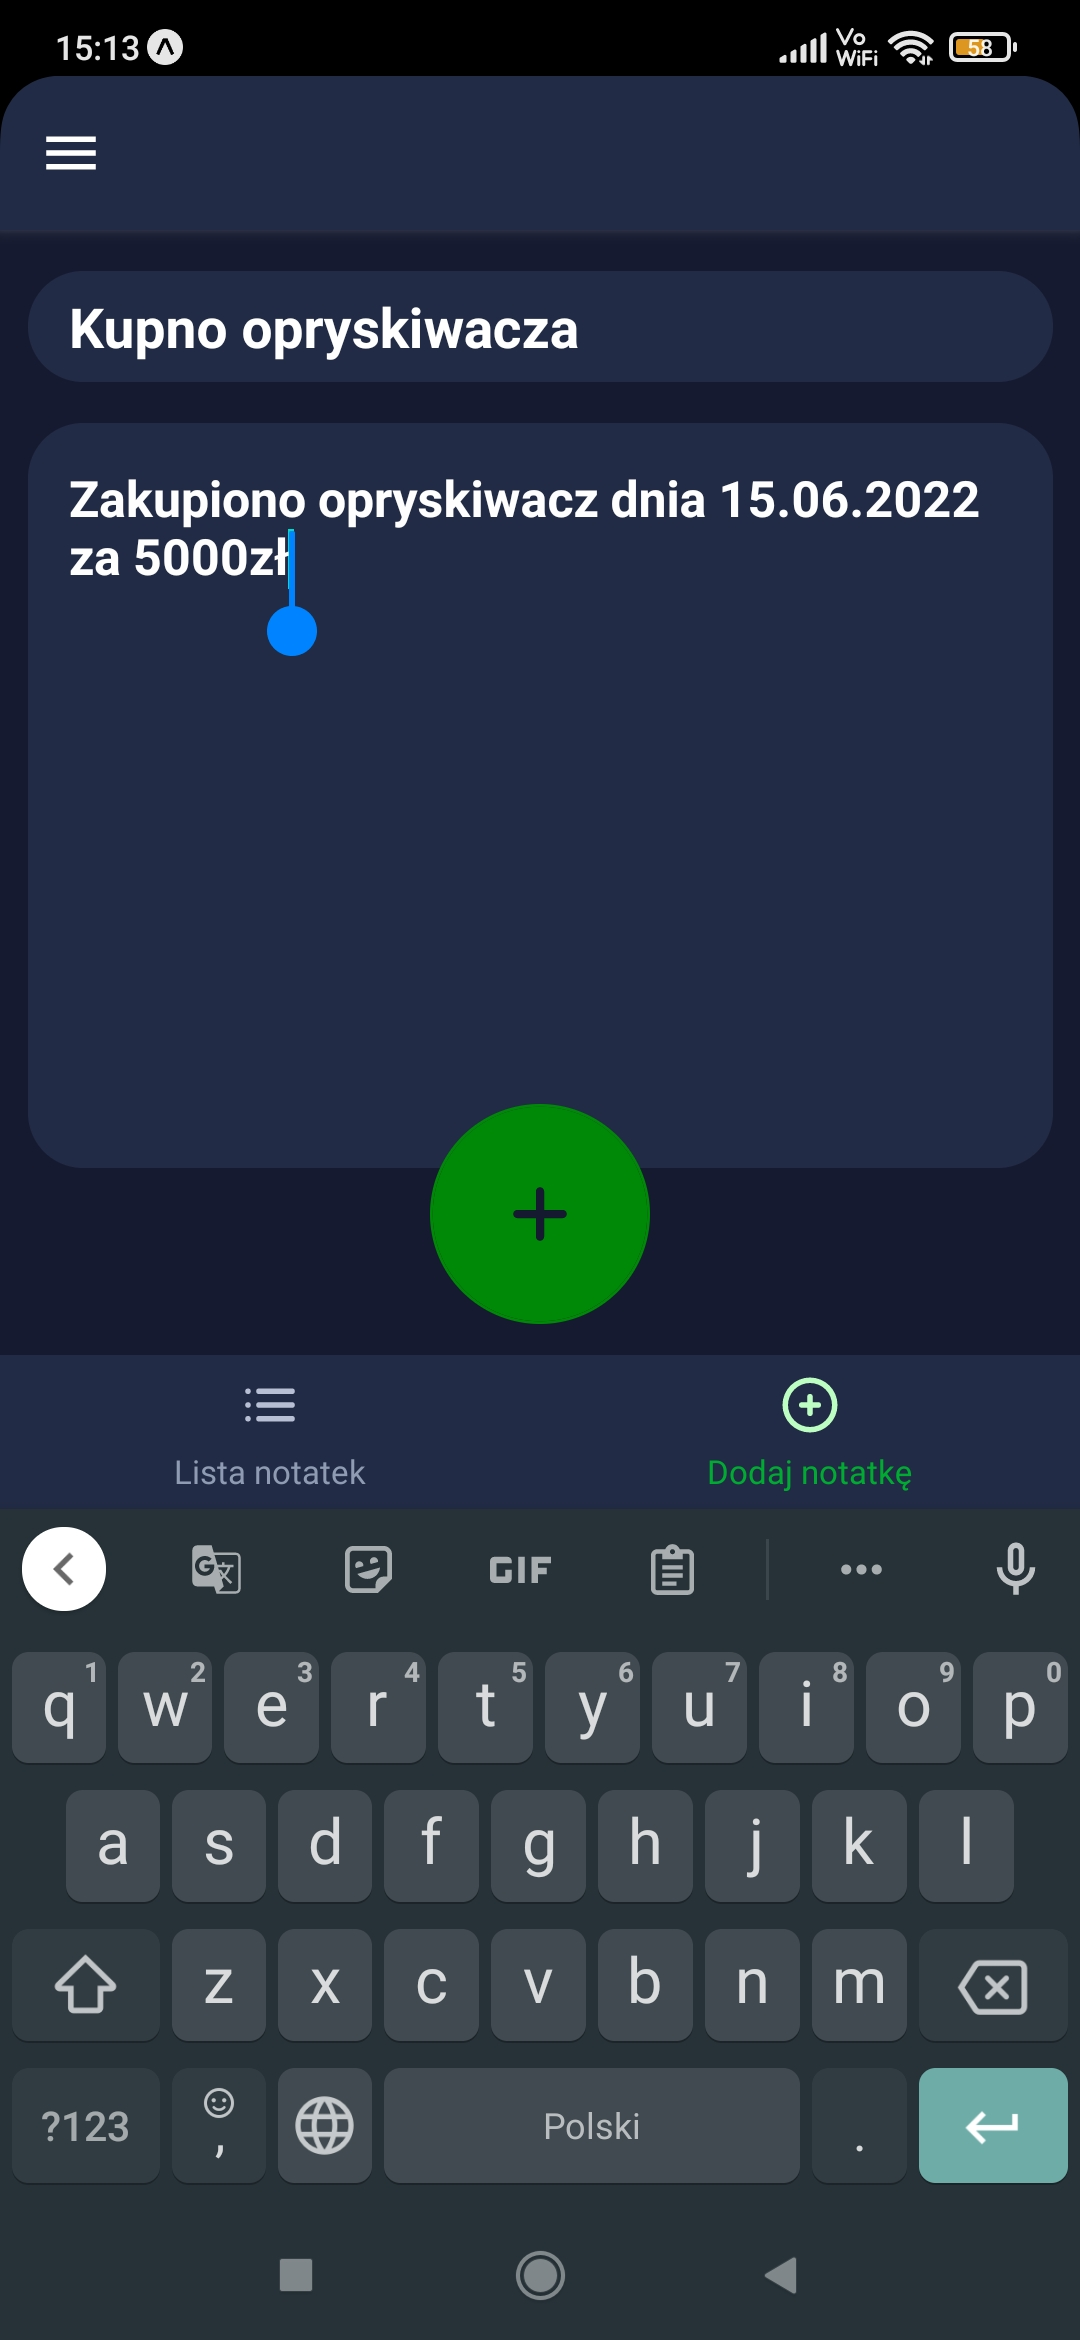
\includegraphics[width=0.8\textwidth]{grafika/notatki_a.jpg}
			\caption{Dodawanie notatek}
		\end{subfigure}%
		\begin{subfigure}{.5\textwidth}
			\centering
			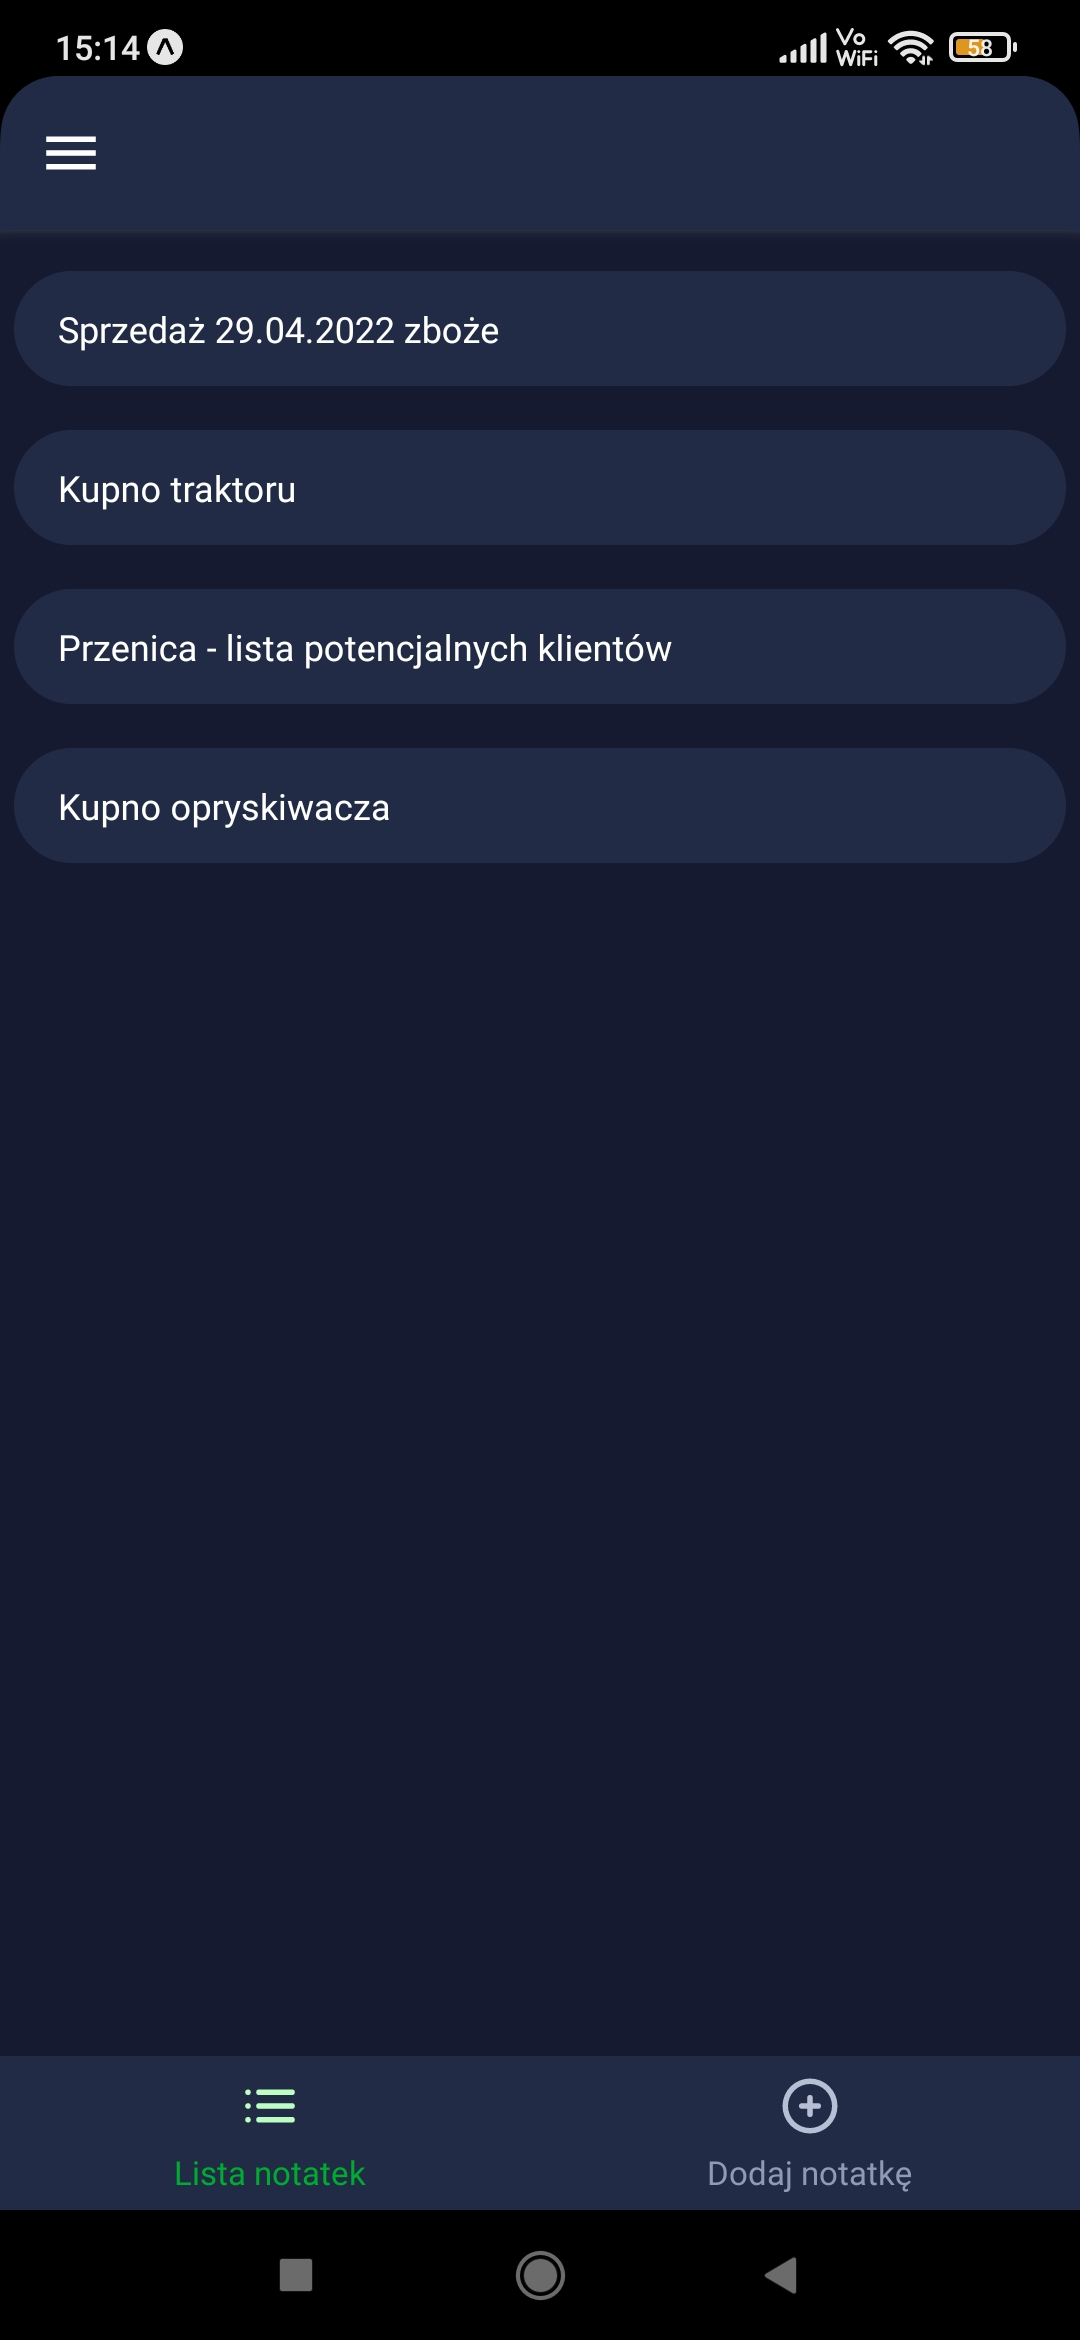
\includegraphics[width=0.8\textwidth]{grafika/notatki_b.jpg}
			\caption{Lista notatek}
		\end{subfigure}
		\caption{Zrzuty ekranu funkcji "Notatki"}
	\end{figure}
	
	Prosty interfejs pozwala na łatwe wyszukiwanie i przeglądanie listy notatek. W celu wyświetlenia zapisanych informacji wystarczy kliknąć na wybrany element listy. Użytkownik zostanie wtedy przeniesiony do widoku szczegółowego gdzie będzie mógł czytać lub usuwać wybrane notatki (Rysunek 3.5).
	
	\begin{figure}[H]
		\centering
		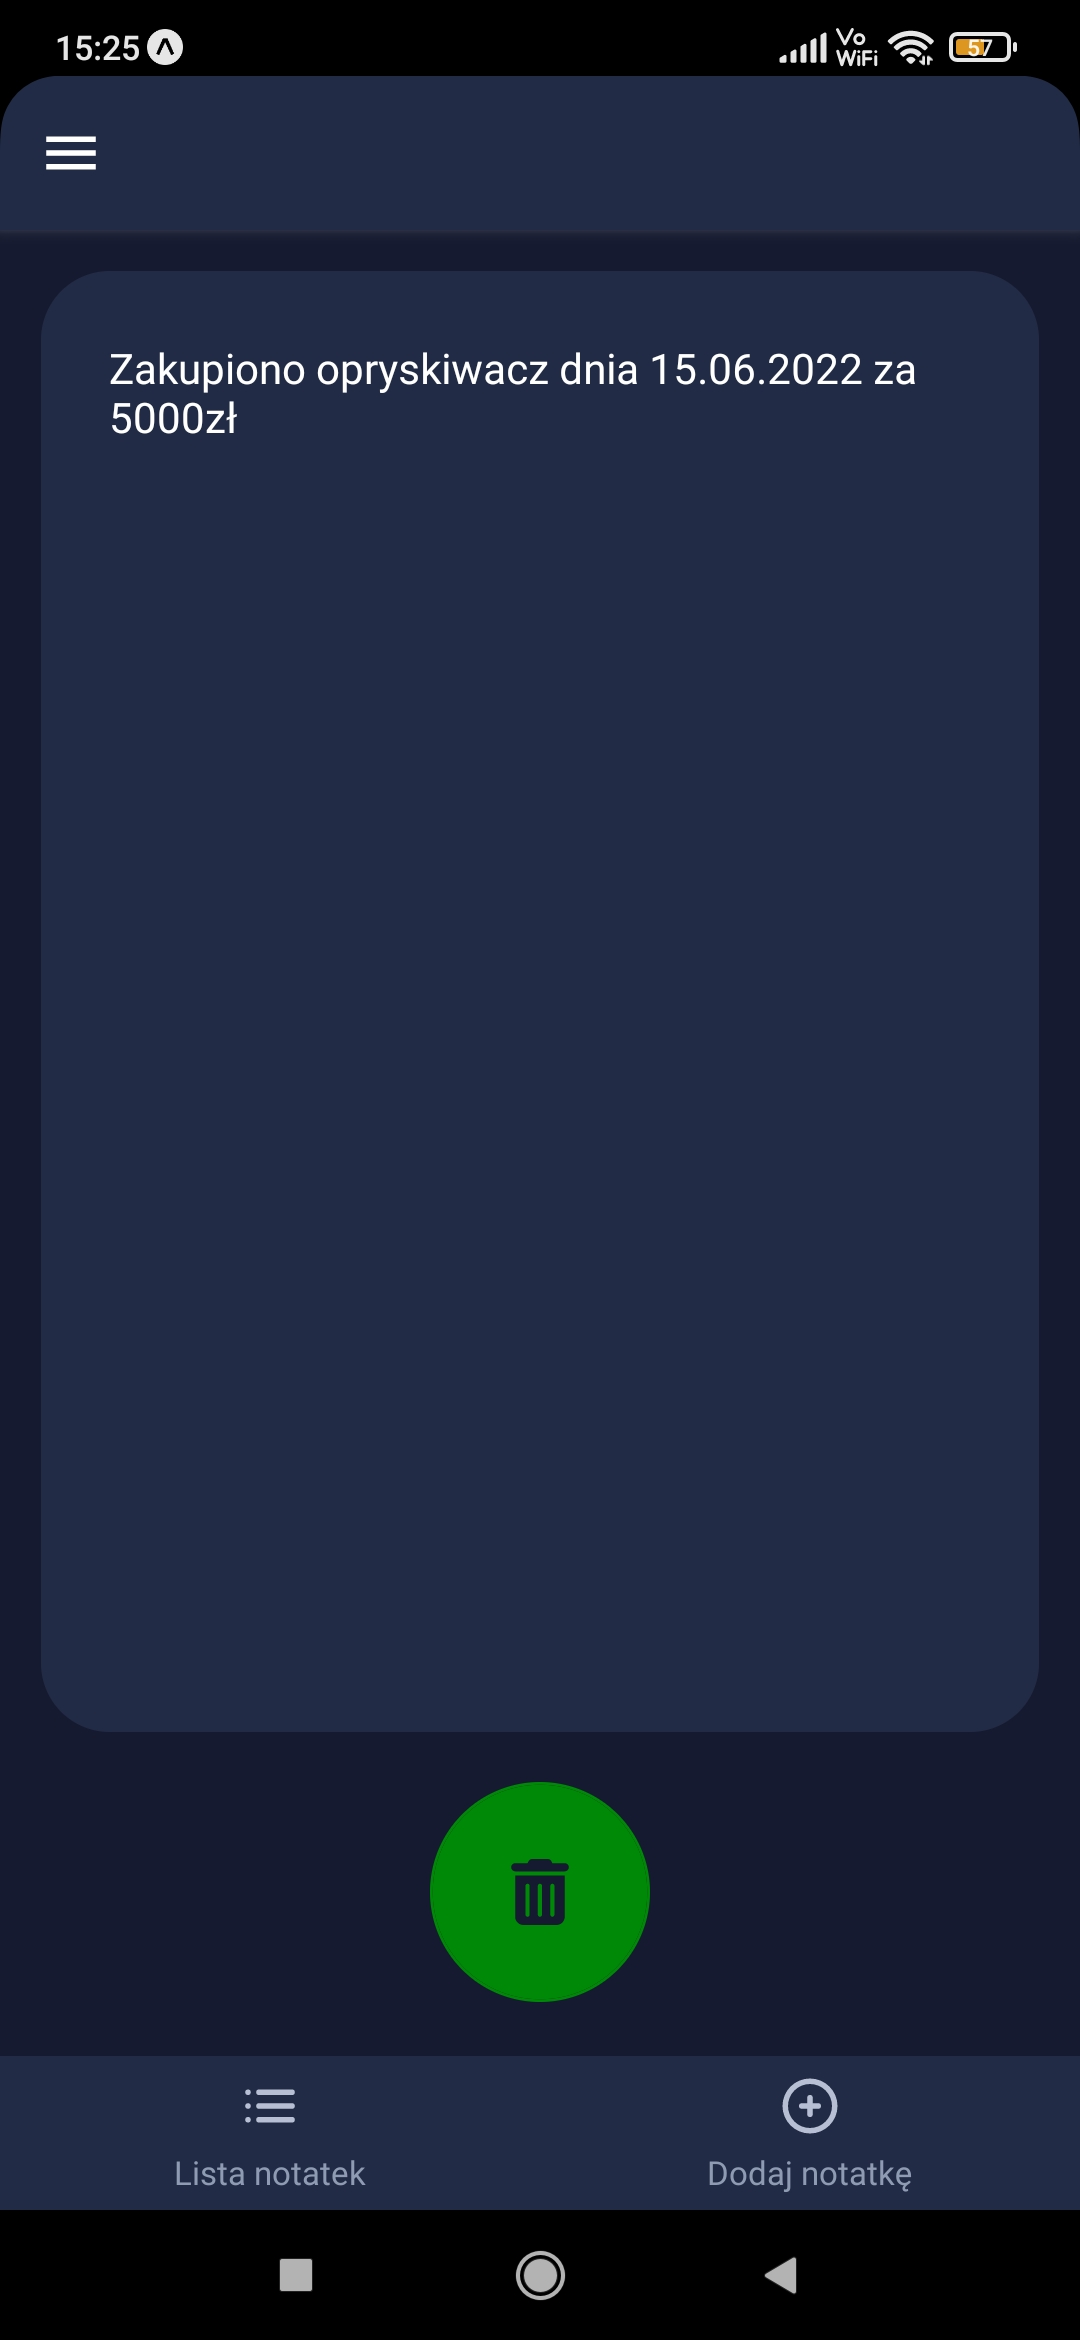
\includegraphics[width=0.5\textwidth]{grafika/notatki_c.jpg}
		\caption{Szczegółowy widok notatek}
	\end{figure}
	
	\subsection{Kalkulator wysiewu zbóż}
	\ \ \ \
		Trzecią z kolei funkcjonalnością jest kalkulator wysiewu zbóż. Jego głównym celem jest obliczanie masy wysiewu zboża w kilogramach na hektar w celu otrzymania optymalnej ilości, którą rolnik musi zastosować przy zasiewaniu pola. Kalkulator wysiewu oblicza ilość wysiewu zboża za pomocą poniższego wzoru (3.1)
		
	\begin{equation}
		\textrm{\textbf{\textit{Ilość wysiewu}}} = \frac{\textbf{MTZ}*\textbf{Obsada}}{\textrm{\textit{\textbf{Siła kiełkowania}}}}
	\end{equation}
	\\
	\begin{description}
		\item[MTZ] - masa tysiąca ziaren, określana w gramach
		\item[Obsada] - jest to ilość roślin na jednostce powierzchni, określana jako sztuka/$ m^{2} $ 
		\item[Siła kiełkowania] - określona dla nasion kwalifikowanych, określana w \% 
	\end{description}
	
	Funkcja kalkulatora wysiewu składa się z dwóch widoków: widoku kalkulatora oraz widoku z informacjami. Pierwszy widok pozwala użytkownikowi na wprowadzenie oraz obliczenie ilości wysiewu. Funkcja ta zawiera w sobie prostą walidację uniemożliwiającą użytkownikowi wprowadzenia niepoprawnych lub pustych danych. W przypadku poprawnego wpisania wszystkich danych i naciśnięciu przycisku oblicz otrzymamy wynik w kg/ha (Rysunek 3.6a). W przeciwnym wypadku aplikacja poinformuje nas o błędnie wpisanych danych.  Drugi widok natomiast pełni funkcję legendy, która daje informacje o potrzebnych do obliczeniach zmiennych. Dodatkowo dla masy tysiąca ziaren stworzona została lisa gatunków zbóż razem z ich MTZ, a dla siły kiełkowania podany został sposób na określenie tej wartości (Rysunek 3.6b)
	
	\begin{figure}[H]
		\centering
		\begin{subfigure}{.5\textwidth}
			\centering
			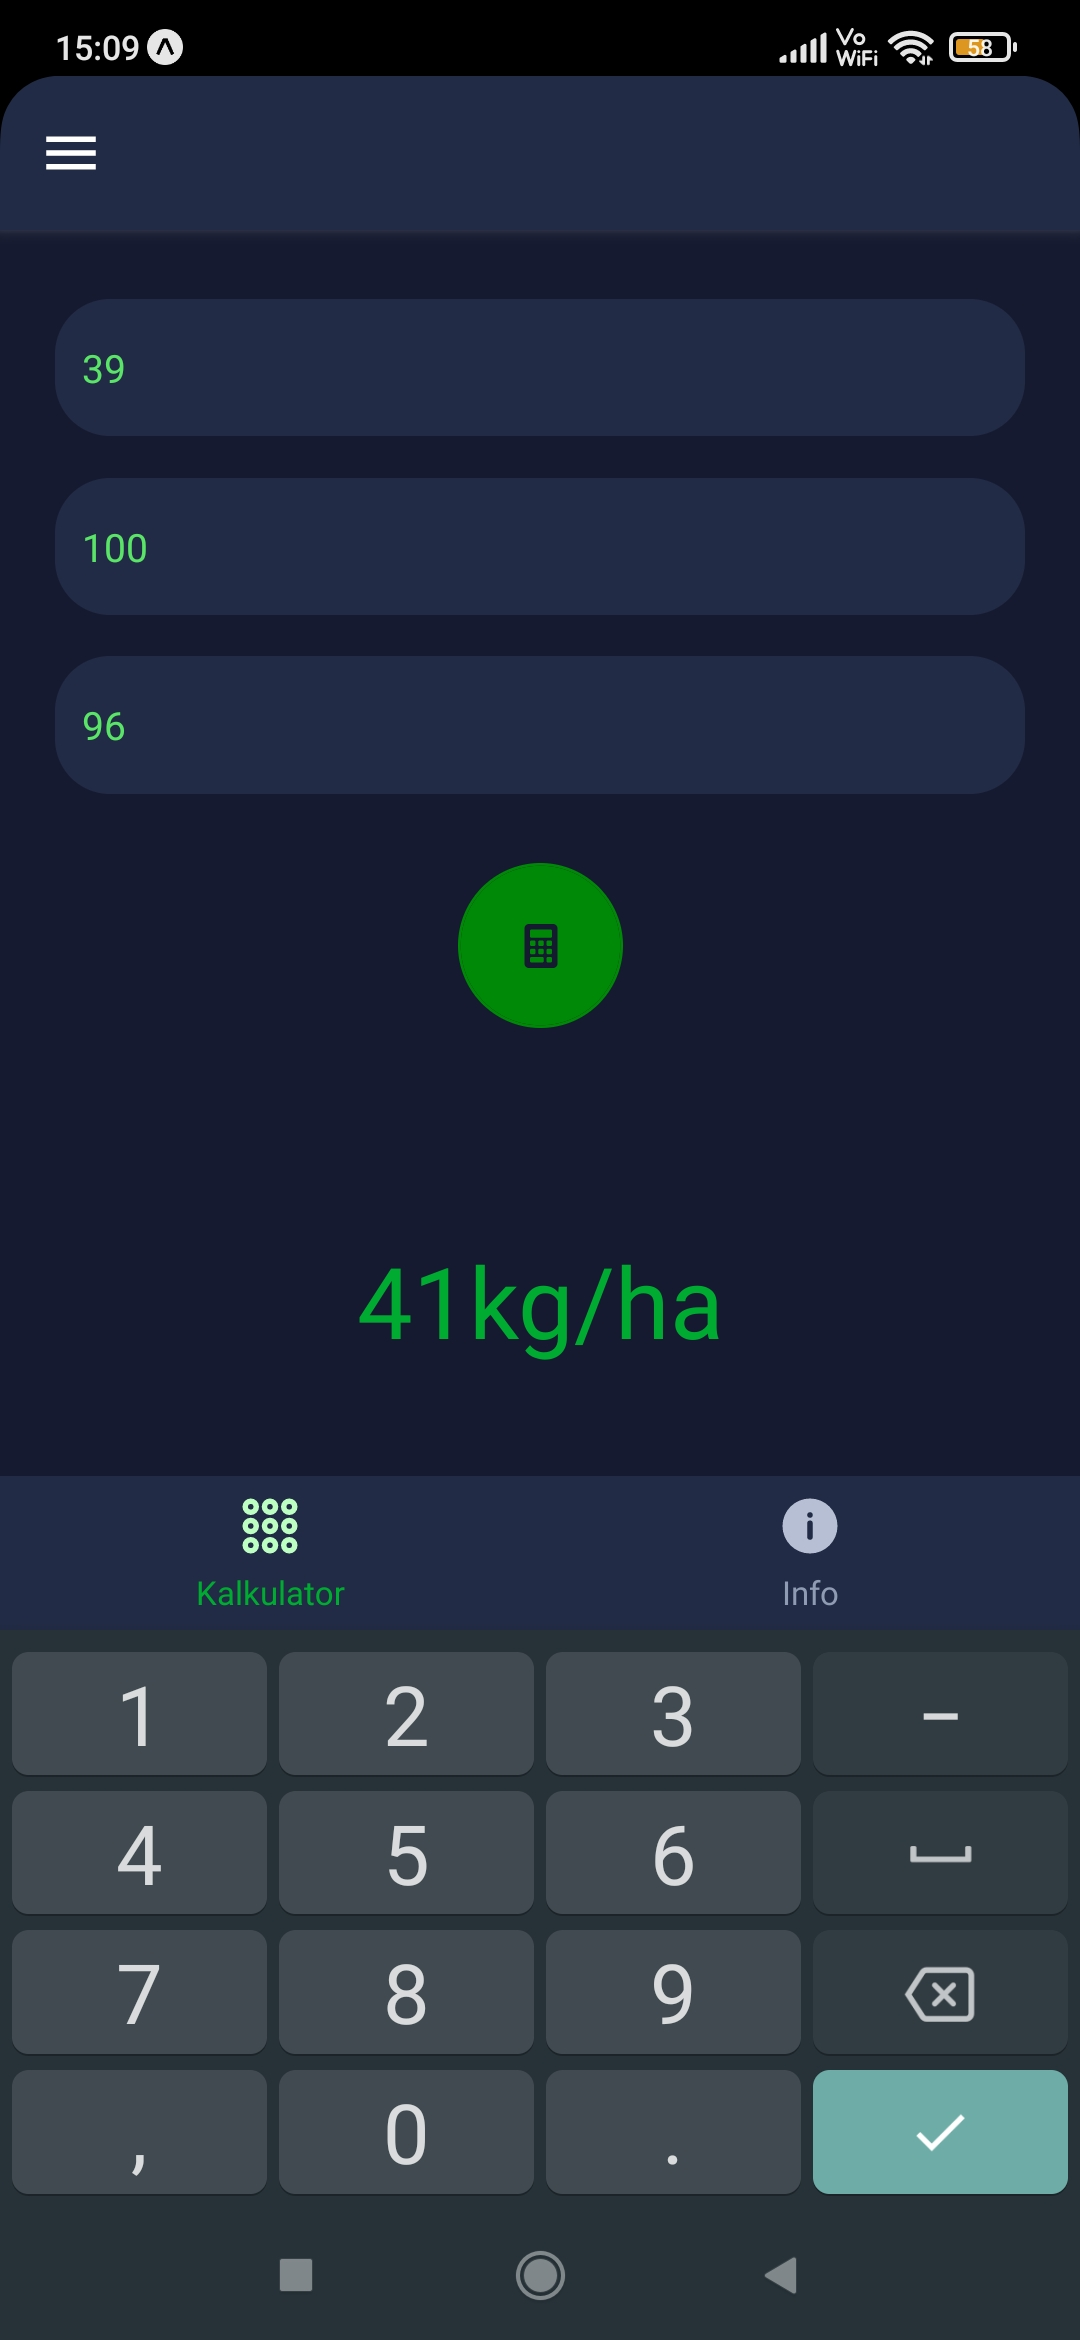
\includegraphics[width=0.8\textwidth]{grafika/kal_a.jpg}
			\caption{Widok kalkulatora}
		\end{subfigure}%
		\begin{subfigure}{.5\textwidth}
			\centering
			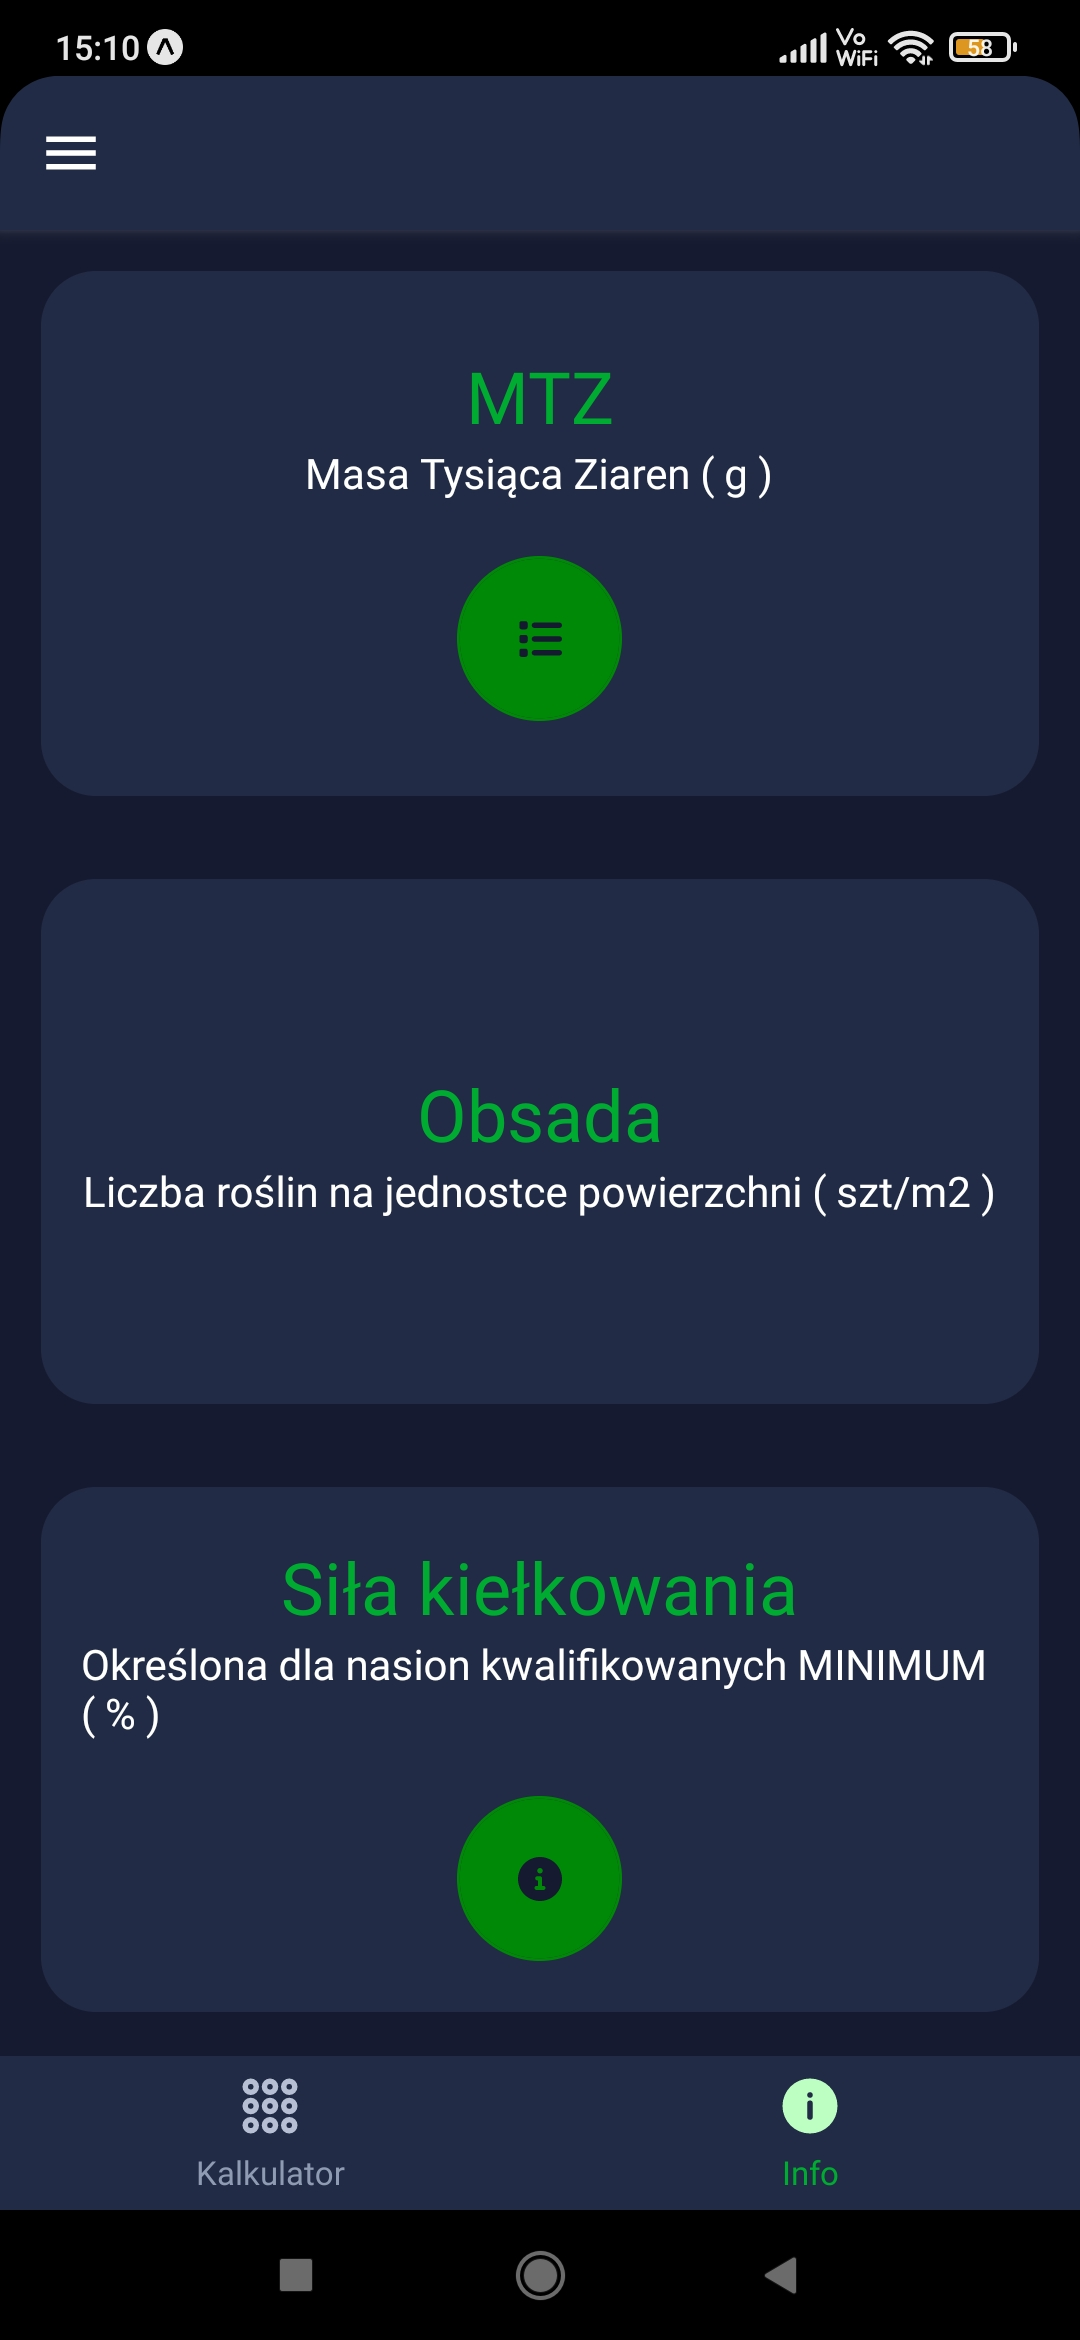
\includegraphics[width=0.8\textwidth]{grafika/kal_b.jpg}
			\caption{Widok informacji}
		\end{subfigure}
		\caption{Zrzuty ekranu funkcji "Kalkulator wysiewu zbóż"}
	\end{figure}
	
	\subsection{Wyszukiwarka środków ochrony roślin}
	\ \ \ \
		Przedostatnią już funkcjonalnością w aplikacji Agro4Farm jest wyszukiwarka środków ochrony roślin. Jest to bardziej złożona funkcjonalność składająca się z wyszukiwarki ochrony roślin stworzonej po stronie aplikacji oraz stworzonego na potrzeby aplikacji interfejsu API łączącego się ze spisem środków ochrony roślin. Wyżej wspomniany interfejs programowania aplikacji został stworzony zgodnie z zasadą projektowania REST (ang: representational state transfer).
		
		\newpage
		
		REST API działa na zasadzie wysyłania żądań HTTP. Dzięki temu możliwe jest wykonywanie podstawowych operacji CRUD (ang: create, read, update, delete) w bazie czyli tworzenie, odczytywanie, zmiana oraz usuwanie danych. W przypadku wysłania zapytania interfejs API zwraca użytkownikowi odpowiednie dane, które zazwyczaj zwracane są w formacie JSON lub XML (Rysunek 3.7) \cite{ref14}.
	
		\begin{figure}[H]
			\centering
			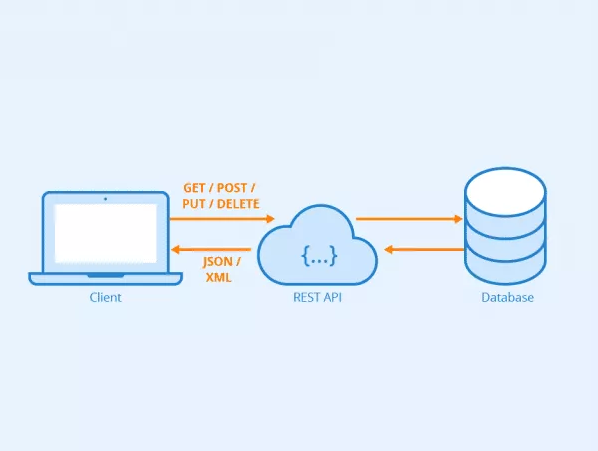
\includegraphics[width=0.9\textwidth]{grafika/restapi.png}
			\caption{Przykładowy schemat działania REST API}
		\end{figure}
	
		API wyszukiwarki środków ochrony roślin do połączenia się z bazą danych używa PRISMA ORM które automatycznie generuje modele oraz wykonuje migracje. Na potrzeby aplikacji interfejs API zwraca dane w zależności od tego jakiego filtru użytkownik używa. Aplikacja pozwala na wyszukiwanie środków ochrony roślin po nazwie produktu, nazwie choroby lub szkodnika oraz po nazwie uprawy, do której ów środek jest stosowany. Dane o konkretnych środkach zwracane są w formacie JSON.
		
		\newpage
		
		\begin{lstlisting}[caption=Kod API filtru wyszukiwania po nazwie uprawy]
			import { PrismaClient } from "@prisma/client"
			import NextCors from 'nextjs-cors'
			import { NextApiRequest, NextApiResponse } from "next"
			
			const prisma = new PrismaClient()
			
			export default async function handle(req: NextApiRequest, res: NextApiResponse) {
				// Wartosc wprowadzona w wyszukiwarce, nazwa uprawy 
				let {query: {name}} = req
				
				await NextCors(req, res, {
					methods: ['GET'],
					origin: '*',
					optionsSuccessStatus: 200,
				})
				// Zapytanie do bazy
				const posts = await prisma.sor.findMany({
					where: {
						uprawa: {
							contains: name as string,
							mode: 'insensitive'
						}
					},
				})
				// Wyslanie odpowiedzi
				res.status(200).json(posts)
			}
		\end{lstlisting}
	
		Aby skorzystać z opcji wyszukiwania użytkownik musi wpisać frazę, którą chcę wyszukać, wybrać odpowiedni filtr i nacisnąć przycisk wyszukiwania. Po otrzymaniu odpowiedzi dane wyświetlane są w postaci listy przesuwanej. Poszczególne elementy zawierają podstawowe informacje o środku ochronnym (Rysunek 3.8a). Po kliknięciu w wybrany element listy zostają wyświetlone szczegółowe informacje o produkcie, gdzie użytkownik ma możliwość wyszukania ofert dla danego produktu lub zapisanie go jako zakupionego (rys 3.8b).
		
		\begin{figure}[H]
			\centering
			\begin{subfigure}{.5\textwidth}
				\centering
				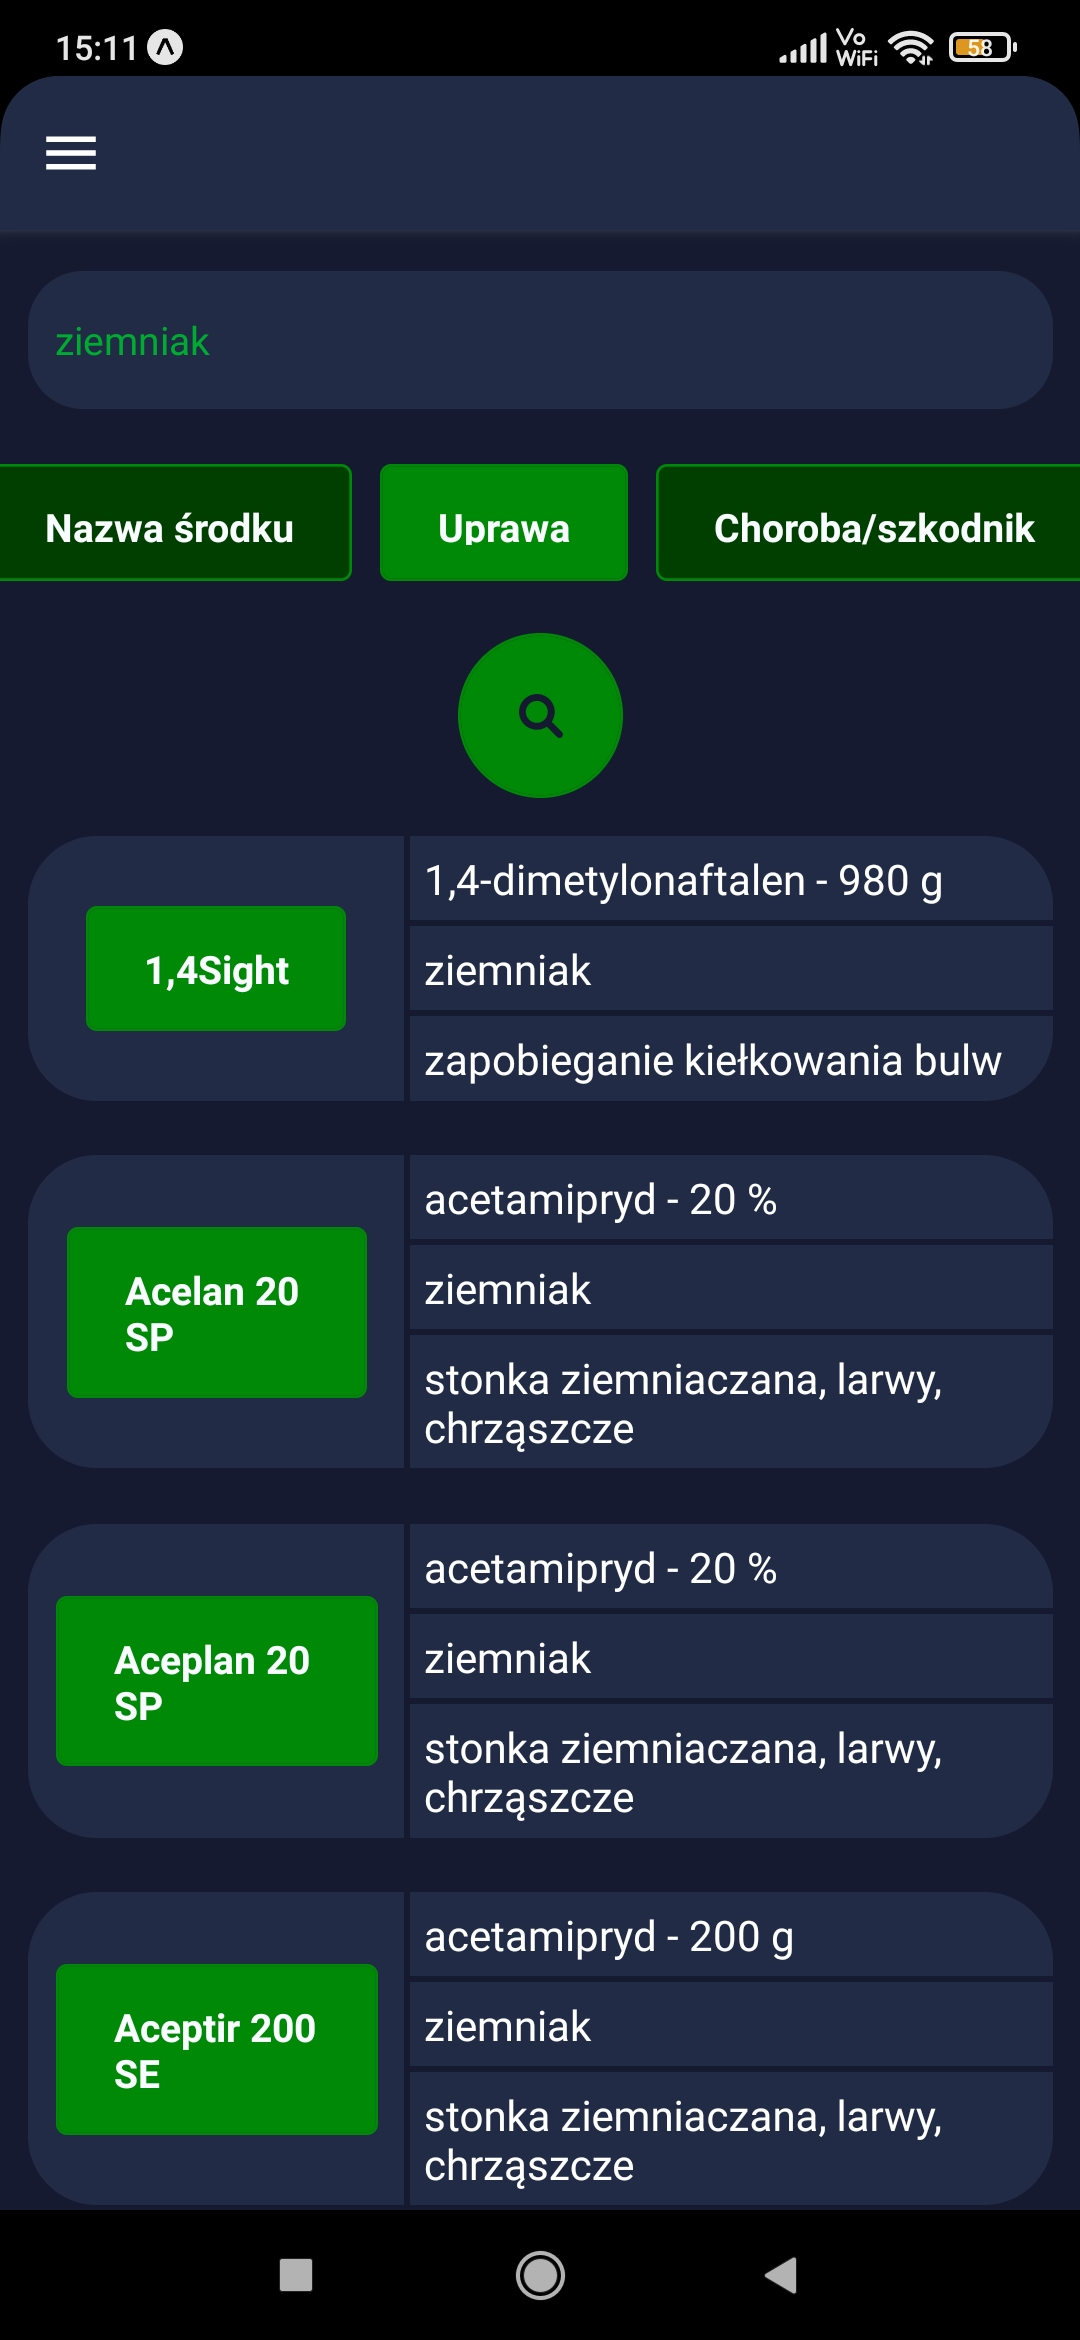
\includegraphics[width=0.8\textwidth]{grafika/wysz_a.jpg}
				\caption{Widok wyszukiwarki}
			\end{subfigure}%
			\begin{subfigure}{.5\textwidth}
				\centering
				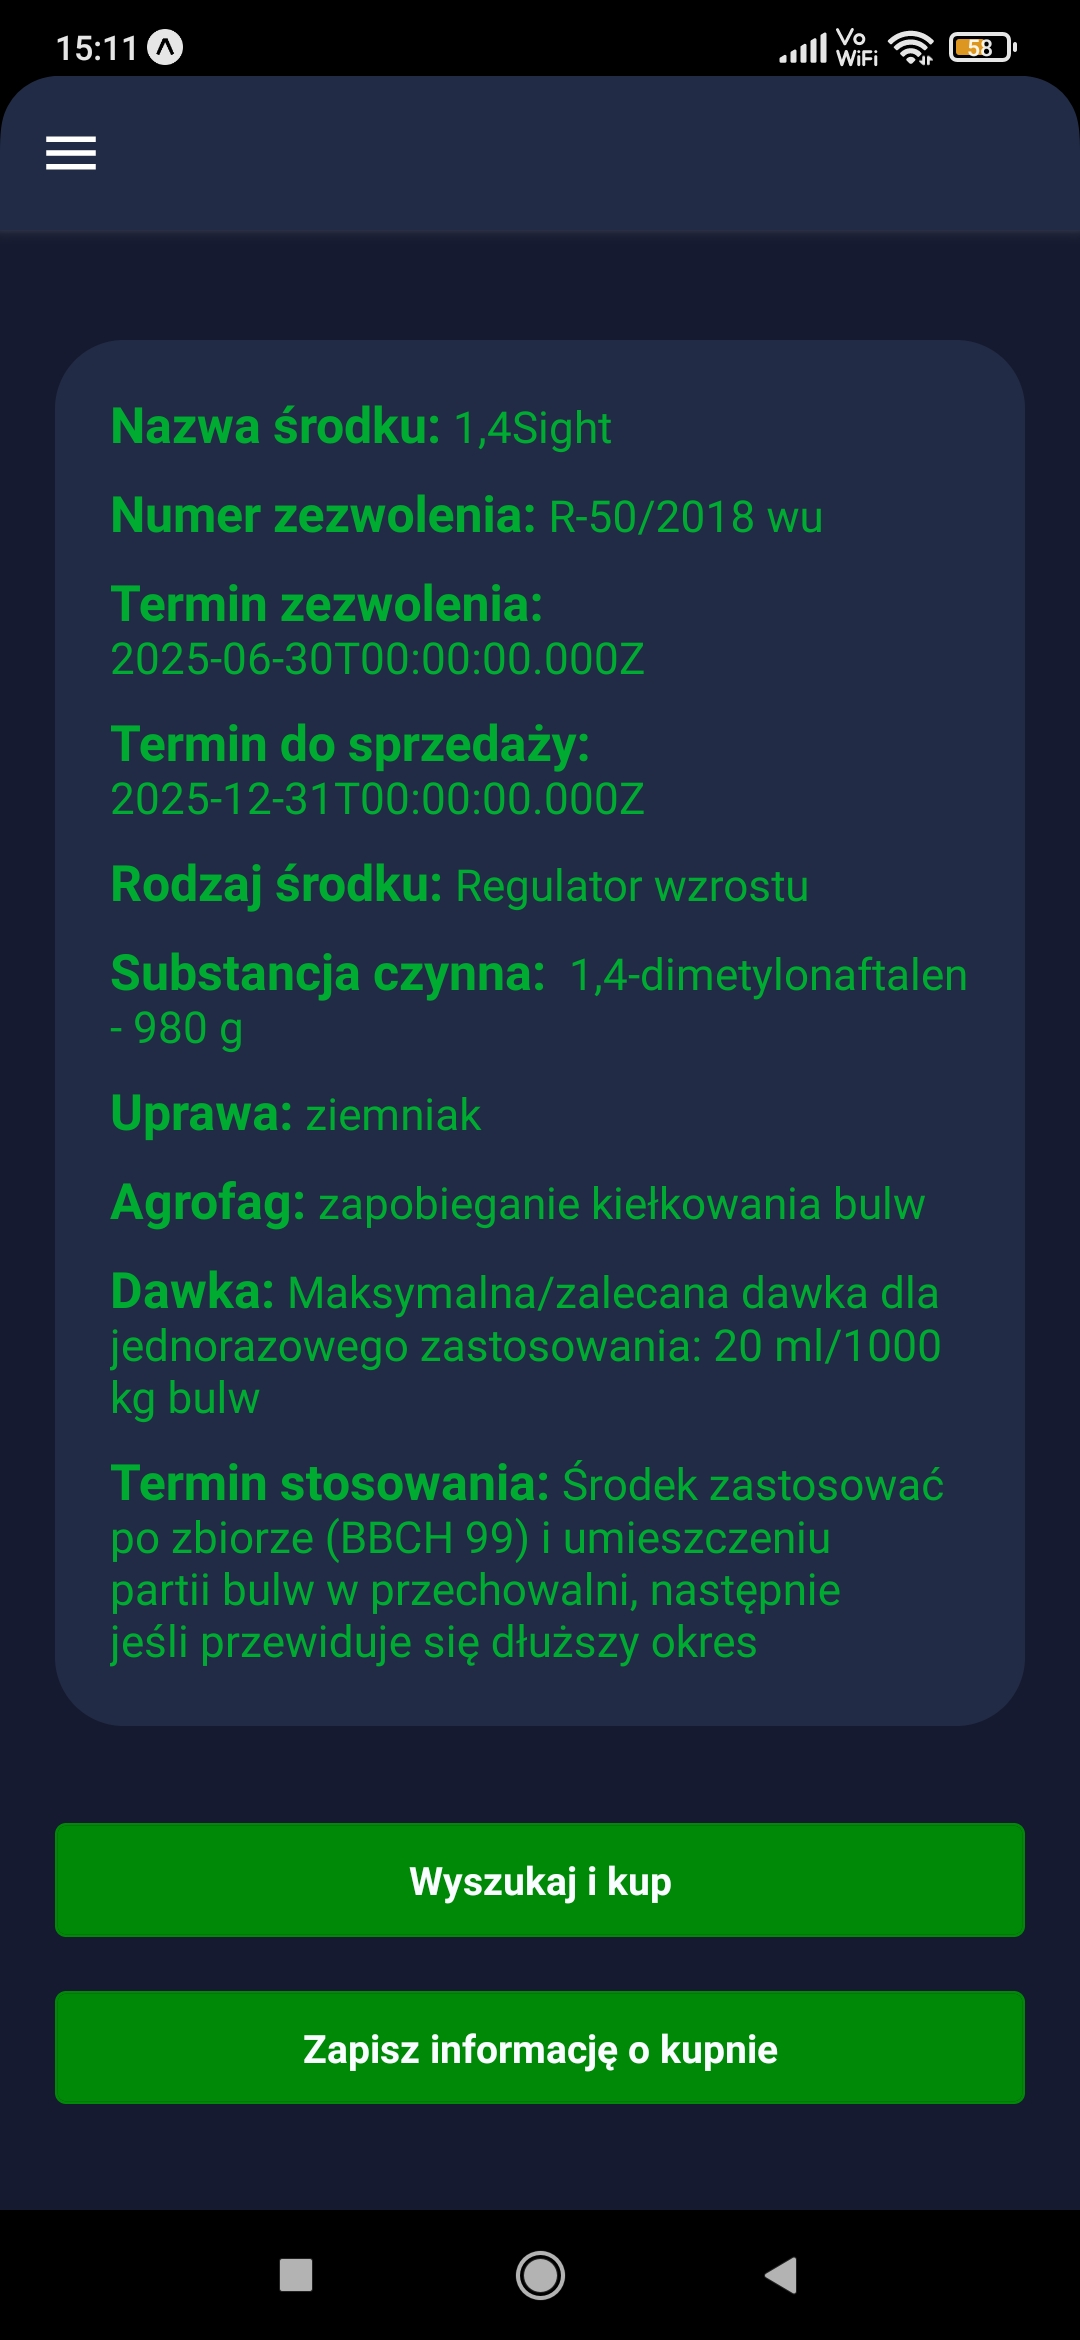
\includegraphics[width=0.8\textwidth]{grafika/wysz_b.jpg}
				\caption{Widok szczegółów}
			\end{subfigure}
			\caption{Zrzuty ekranu funkcji "Wyszukiwarka środków ochrony roślin"}
		\end{figure}
	
		Wyżej wspomniane funkcje, czyli kupno produktu oraz zapisanie informacji o kupnie są kluczowymi funkcjonalnościami tej wyszukiwarki. W aplikacjach rolniczych tego typu brakuje właśnie takich rozwiązań, które z pewnością ułatwiłyby pracę oraz zaoszczędziły czas rolnika. Pierwsza funkcja automatycznie przenosi użytkownika do strony gdzie jest w stanie zakupić dany produkt. Druga z nich natomiast wykorzystuje wspomnianą już wcześniej w tej pracy funkcjonalność "Notatki". 
		
		\newpage
		
		Jeżeli użytkownik ma zamiar zakupić dany produkt może za pomocą przycisku zapisać informację o kupnie danego produktu razem z aktualną datą. Funkcja ta jest o tyle przydatna, gdyż coraz częściej w gospodarstwach wymagane jest prowadzenie ewidencji zakupów i sprzedaży.
		
		\begin{figure}[H]
			\centering
			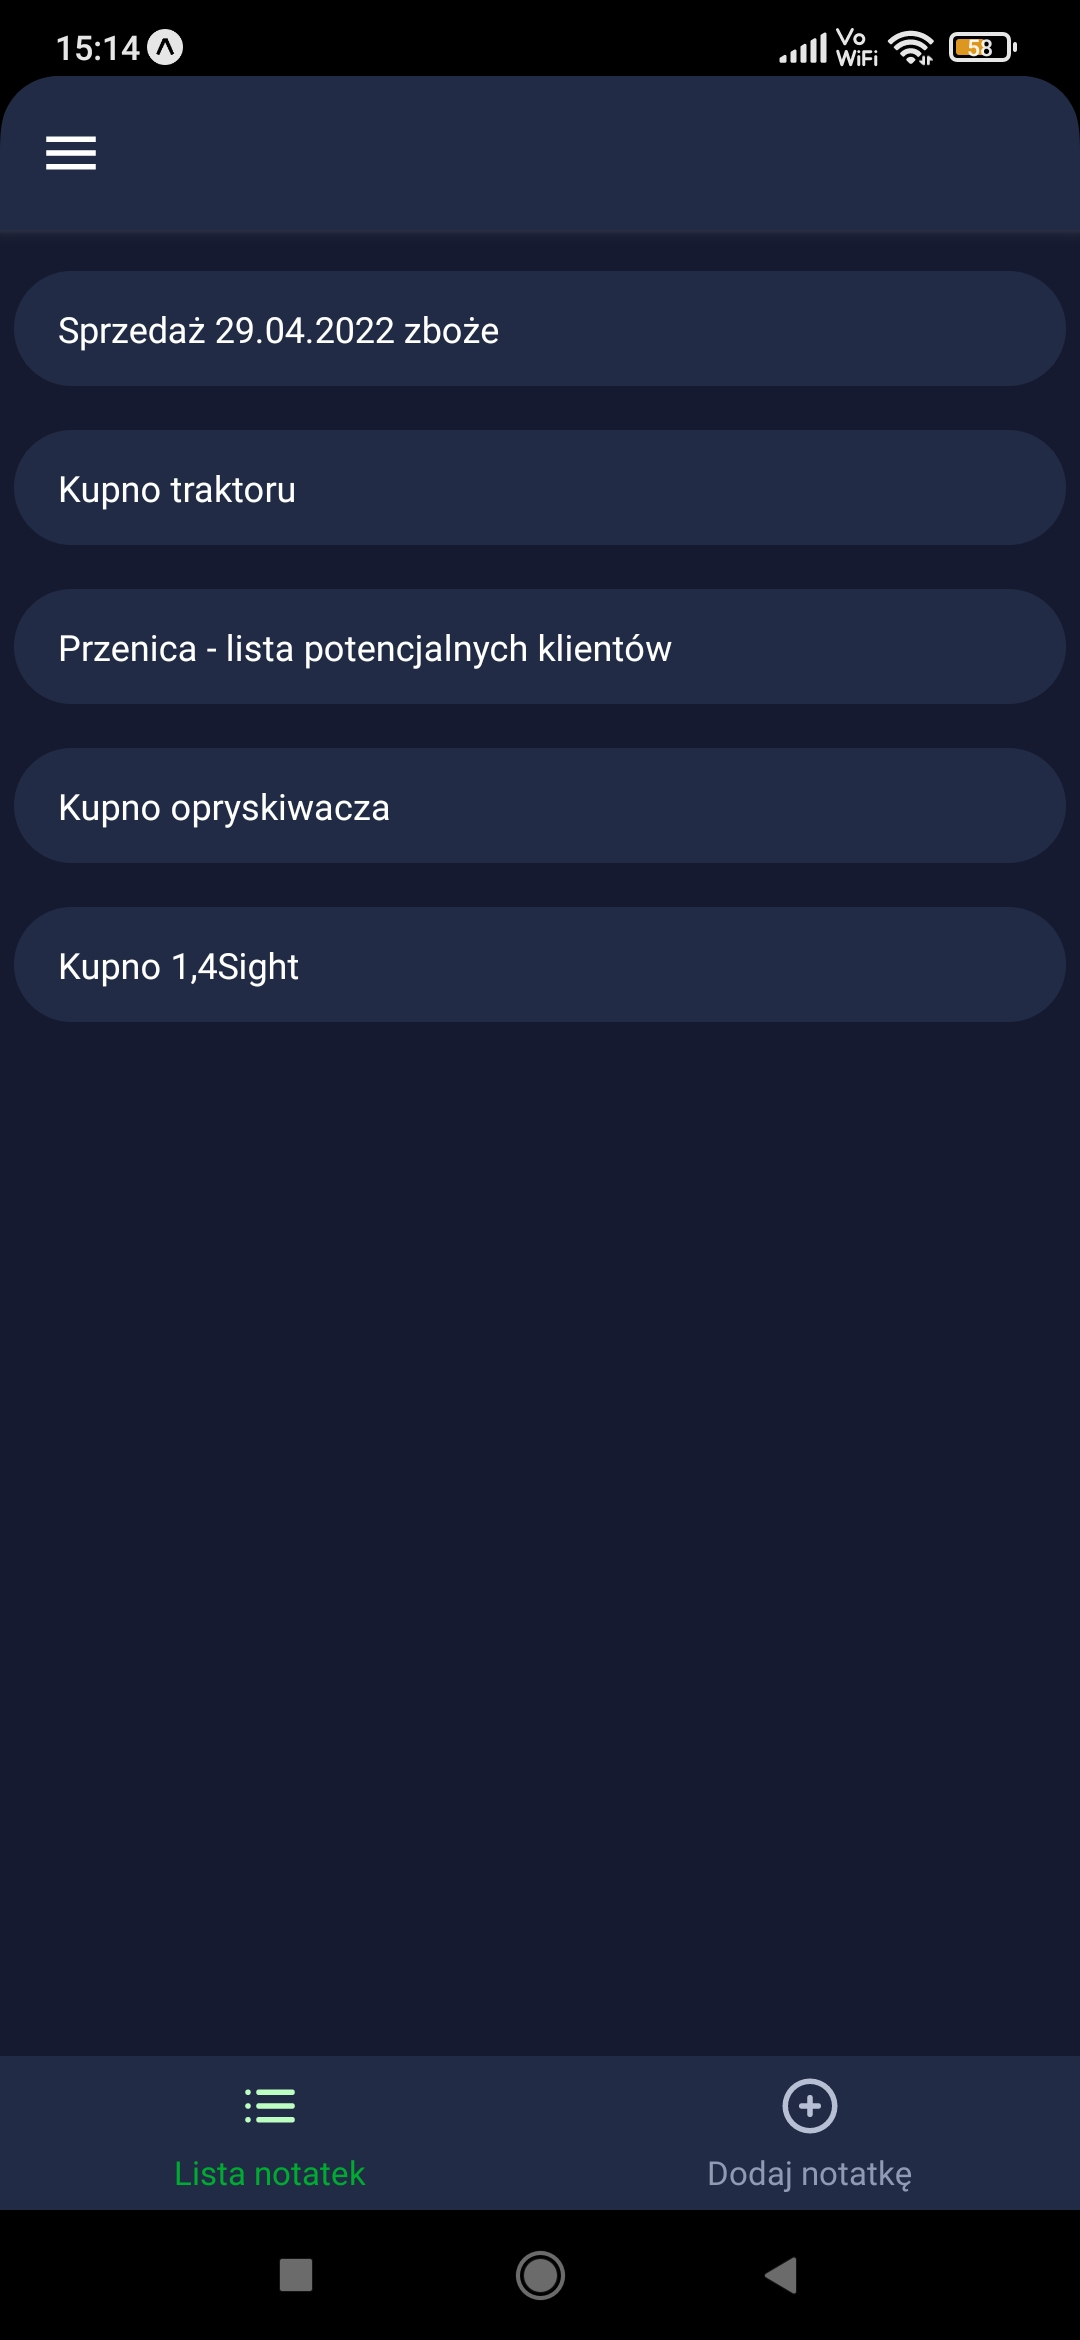
\includegraphics[width=0.55\textwidth]{grafika/wysz_c.jpg}
			\caption{Notatki po dodaniu informacji o kupnie produktu}
		\end{figure}
	
	\subsection{Przewidywanie terminów pracy i nawożenia}
	\ \ \ \
		Piątą i ostatnią możliwością tej aplikacji jest funkcja pozwalająca na przewidywanie optymalnych terminów nawożenia oraz pracy na roli. Jest to kolejny przykład opcji, która występuje w aplikacjach rolniczych rzadko lub też wcale. Funkcja ta jest o tyle przydatna gdyż praca na roli w głównej mierze zależna od warunków pogodowych. Użytkownik na podstawie przewidywań aplikacji jest wstanie zaplanować swoją prace na najbliższe dni. Aplikacja używa tego samego interfejsu API funkcja "Pogoda" z tą różnicą, że dane pogodowe pobierane są na okres najbliższego tygodnia i jest w stanie przewidzieć trzy typy terminów prac, czyli:
		
		\begin{description}
			\item[Termin optymanly] - jest to dzień, w którym warunki pogodowe są perfekcyjne do nawożenia upraw lub pracy. Termin ten oznaczany jest symbolem zielonej łapki w górę.
			\item[Termin dobry] - jest to dzień w którym stan pogody jest na poziomie dobrym, ale nie spełnia wszystkich warunków wymaganych dla stanu optymalnego. Jest to termin pozwalający na prace polowe, ale nie koniecznie na nawożenie upraw. Termin ten oznaczany jest symbolem żółtej łapki w górę.
			\item[Termin nieoptymalny] - jest to dzień w którym warunki pogodowe nie pozwalają na nawożenie upraw oraz na pracę w polu. Termin ten oznaczany jest symbolem czerwonej łapki w dół.
		\end{description}
	
		Sprawdzając, czy dany termin pozwala na pracę polowe aplikacja bierze pod uwagę wartości wilgotności powietrza, temperatury, siły wiatru oraz prawdopodobieństwa opadów. Aby dany termin był wyświetlany jako optymalny temperatura powinna zawierać się w zakresie $10-20^{\circ} C$. Wilgotność powietrza musi wynosić około 50 - 80 \%, dla dobrej chłonności nawozów przez glebę. Siła wiatru oraz prawdopodobieństwo opadów powinny być na poziomie niskim lub zerowym. Jeżeli jeden z wyżej wymienionych warunków atmosferycznych nieznacznie przekracza któryś z zakresów, termin spada do poziomu dobrego, a w przypadku naprawdę złych warunków pogodowych na przykład: prawdopodobieństwo opadów 50 - 100 \%, bardzo silny wiatr lub zła temperatura, termin spada do poziomu nieoptymalnego. Górna część interfejsu funkcjonalności pokazuje użytkownikowi szczegółowe warunki na aktualny dzień wraz z określeniem czy termin jest optymalny. Dolny panel składa się z listy przewijanej zawierającej predykcje na najbliższy tydzień. Dodatkowo użytkownik na możliwość wyszukania najbliższego optymalnego dnia za pomocą przycisku wyszukiwania (Rysunek 3.10).
		
		\begin{figure}[H]
			\centering
			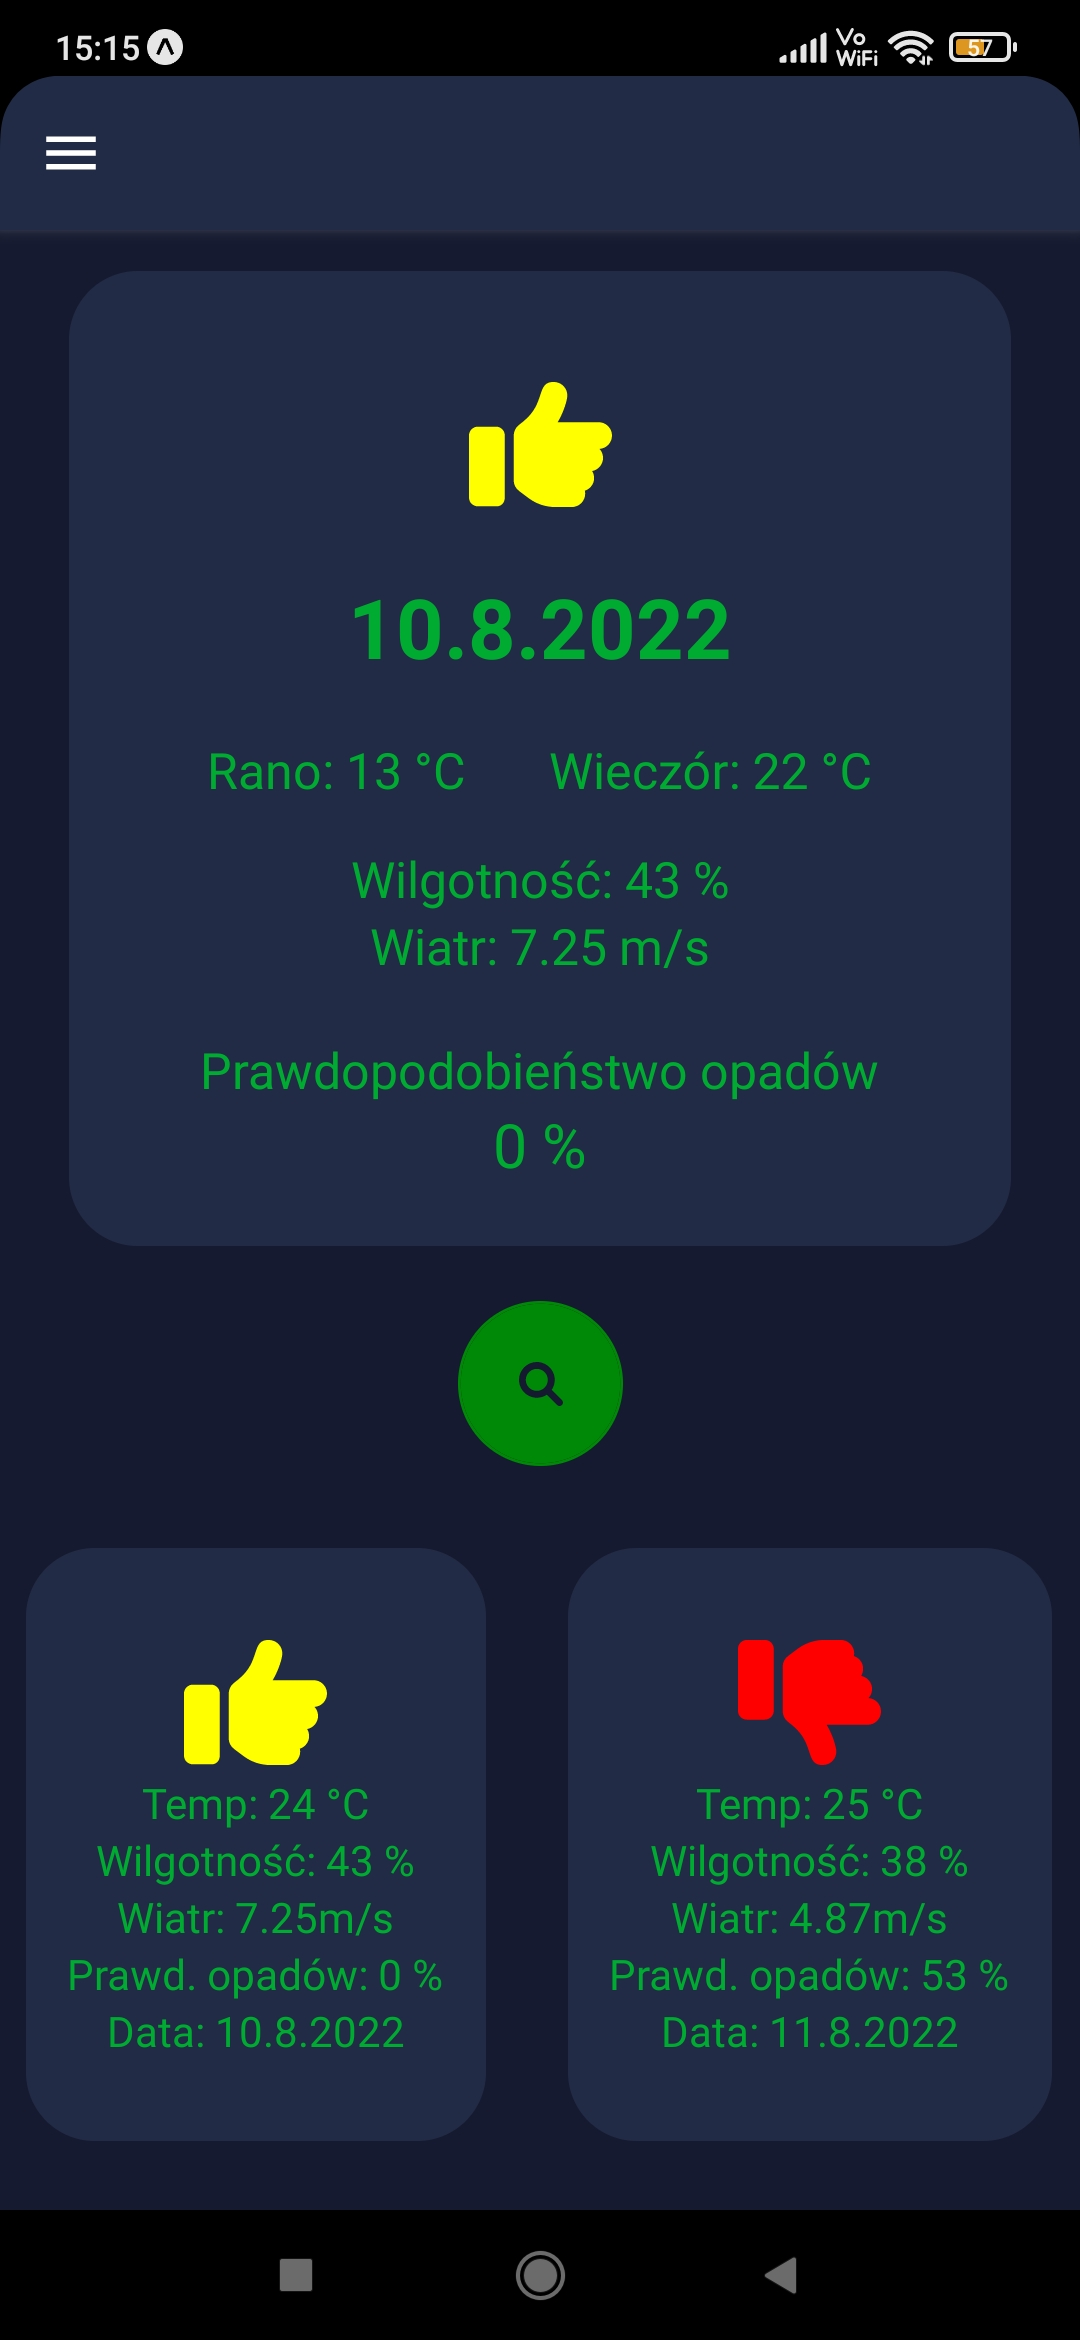
\includegraphics[width=0.48\textwidth]{grafika/pre.jpg}
			\caption{Zrzuty ekranu funkcji "Przewidywanie terminów pracy i nawożenia"}
		\end{figure}
		
	\newpage
	\chapter{Podsumowanie}
	\section{Możliwości dalszego rozwoju aplikacji}
	\ \ \ \
	Mimo to, że prace nad aplikacją zostały zakończone, nie oznacza to, że nie istnieje możliwość jej usprawnienia. Agro4Farm jako aplikacja mobilna może zostać ulepszona pod względem funkcjonalności jak i interfejsu użytkownika. Niektórymi zmianami, które usprawniłyby aplikację są:
	
	\begin{description}
		\item[System logowania i rejestracji -] funkcja ta usprawniłaby identyfikację użytkownika oraz pozwoliłaby na przechowywanie szczegółowych informacji zapisanych w aplikacji poza urządzeniem.
		\item[Aplikacja webowa, aplikacja na komputery osobiste -] nie można zaprzestać na jedynie wersji mobilnej. W dzisiejszych czasach aplikacje są pisane z myślą o wieloplatformowości, co daje użytkownikowi większą swobodę użycia.
		\item[Wersja na urządzenia z systemem iOS -] aktualnie aplikacja jest skierowana na urządzenia z systemem android, lecz nic nie stoi na przeszkodzie, aby wydać aplikację na urządzenia z systemem iOS.
		\item[Automatyczne aktualizacje bazy danych -] baza środków ochrony roślin pobierana ze strony polskiego rządu musi być aktualizowana ręcznie. W przyszłych wersjach istnieje możliwość wprowadzenia automatycznych aktualizacji bazy.
		\item[Motywy -] coraz więcej aplikacji wprowadza w swoich ustawieniach możliwość zmiany motywów. Dla użytkownika taka opcja byłaby przyjemną zmianą estetyczną pozwalającą na większą swobodę.
	\end{description}
	
	
	\section{Zakończenie}
	\ \ \ \
	Celem przedstawionej pracy było zaprojektowanie aplikacji mobilnej, której zadaniem było ułatwienie oraz organizacja pracy na roli. Pomimo wielu zmagań i przeciwności, udało się pomyślnie stworzyć rozwiązanie, które może zmienić życie wielu rolników. W pracy dokładnie przedstawiono dostępne w aplikacji funkcjonalności wraz z użytymi w nich technologiami. Przedstawiono krótkie fragmenty kodu aplikacji dla poszczególnych funkcji. Za pomocą zrzutów ekranu zaprezentowano wygląd całej aplikacji oraz jej poszczególnych funkcji. 
	
	Oprócz tego przedstawiono krótką historię urządzeń mobilnych oraz opisano używane w nich mobilne systemy operacyjne. Wspomniane zostały również podobne aplikacje dostępne w internecie. Dodatkowo jako zakończenie przedstawiono możliwości rozwoju dla przyszłych wersji aplikacji.
	
	\newpage
	
	\bibliographystyle{IEEEtran}
	\bibliography{./references.bib}
	
	\lstlistoflistings
	
	\listoffigures
	\addcontentsline{toc}{section}{Spis rysunków}
	
\end{document}